\documentclass[11pt]{article}

% ACL style — review mode (anonymous)
\usepackage[review]{acl}

% Fonts and encoding
\usepackage{times}
\usepackage{latexsym}
\usepackage[T1]{fontenc}
\usepackage[utf8]{inputenc}
\usepackage{microtype}
% \usepackage{inconsolata}  % not available in target TeX install

% Math
\usepackage{amsmath}
\usepackage{amssymb}

% Tables and figures
\usepackage{booktabs}
\usepackage{graphicx}
\graphicspath{{figures/}}
\usepackage{subcaption}
\usepackage{multirow}
\usepackage{array}
\usepackage{tabularx}
% \usepackage{adjustbox}  % not available in target TeX install
% \usepackage{placeins}  % not available in target TeX install
% \usepackage{enumitem}  % not available in target TeX install

\title{Acquiescence Is Not Personality: \\ Why Human Psychometric Instruments Fail on Large Language Models}

\author{Anonymous Authors}

\begin{document}
\maketitle

\begin{abstract}
A fast-growing literature scores large language models on validated human personality inventories and feeds the resulting profiles into ``silicon-sample'' surveys and persona-conditioned multi-agent simulations of opinion dynamics, polarisation, and social behaviour. We ask the prior measurement question: when human instruments are administered to LLMs, do they measure anything at all? We administer a 221-item battery (IPIP-NEO-120, SD3, ZKPQ-50-CC, EPQR-A; 17 domains; 63 reverse-keyed items) to 20 chat-tuned LLMs from 8 vendor families under a Default no-persona instruction and all 16 MBTI personas with $k{=}5$ samples per cell at $T{=}0.7$ --- 375{,}700 raw API calls. We then run six standard psychometric validity checks plus a persona stress test. Every check fails. The failures share a single mechanism: a shared acquiescent response style with a directional asymmetry --- positive forward-minus-reverse agree-rate gap on normal items (IPIP $\Delta{=}{+}0.31$) and negative gap on dark-trait items (SD3 $\Delta{=}{-}0.38$). Cronbach's $\alpha$ tracks reverse-item density at Spearman $\rho{=}{-}0.83$ across the 17 domains ($\rho{=}{-}1.0$ on the five IPIP domains); exploratory factor analysis universally collapses the 5 expected Big Five factors into 3 (Tucker's $\varphi{=}0.993$); inter-model variance falls to ${<}1\%$; and $0/320$ $(model, persona)$ pairs achieve measurement invariance against Default. Persona prompts move profiles by ${>}1$ SD per dimension and are $99.7\%$ nearest-centroid recoverable --- enough for \emph{coarse} agent contrast --- but cross-scale coherence is $0.839$ and forward/reverse pair coherence is $0.696$: compliance, not measurement validity. Calibrated against synthetic baselines, LLM alphas hug the Random / Pure-Acquiescence floor and stay far from a Trait+Acquiescence simulation ($\alpha{>}0.99$). The findings impose scope conditions on silicon-sample and persona-agent simulations: coarse persona contrast is reproducible, but trait-grounded simulation of fine-grained psychological mechanisms, conflict dynamics, polarisation, and extreme positions sits on a measurement layer the instruments do not currently support.
\end{abstract}

% ----------------------------------------------------------------------
% Section 1 + 2: Introduction + Related Work (from Step 3)
% ----------------------------------------------------------------------

\section{Introduction}
\label{sec:intro}

Large language models are now being asked the questions psychologists ask people. A fast-growing literature administers validated human personality inventories to chat-tuned LLMs, reports Big Five or Dark Triad scores, and treats the resulting numbers as evidence about an underlying machine character~\citep{miotto2023gpt3,serapio2025psychometric,jiang2023personallm,huang2023psychobench,bodroza2024personality}. These scores in turn feed into proposals to use LLMs as ``silicon samples'' that stand in for human respondents in opinion polling, behavioural experiments, and economic surveys~\citep{argyle2023one,horton2023homo,aher2023using,park2023generative,ferreira2025matching}, and into persona-conditioned multi-agent simulations of opinion dynamics, polarisation, debate, and trust~\citep{chuang2023simulating,cau2025language,chuang2025debate,mannekote2025roleplaying}. The implicit promise is that a model that scores Conscientious on the IPIP-NEO is more conscientious, in some operational sense, than a model that does not --- and, by extension, that a Conscientious-prompted agent will produce trait-consistent behaviour inside a simulated society.

This promise rests on a prior measurement question that is almost never asked: do the human instruments measure anything when they are administered to an LLM? In the human-subjects tradition, an inventory is not trusted until it passes a battery of psychometric checks --- internal consistency, factor structure, convergent validity, and measurement invariance~\citep{cronbach1951coefficient,kaiser1960application,vandenberg2000review}. On LLMs these checks are rarely run; when they appear at all, they typically appear one at a time, on one inventory, on a handful of models~\citep{suhr2025challenging,pelet2025persistent}. \citet{larooij2025validation} make the same observation about generative agent-based modelling: validation, not capability, is the central bottleneck, and current LLM-driven social simulations rely on face validity rather than measurement-grounded calibration.

For a human inventory to measure an LLM ``trait,'' four conditions would need to hold: cross-situational consistency (responses covary across items targeting the same construct, regardless of wording direction), temporal stability, convergent-discriminant structure, and behavioural correspondence. Our audit tests the first and third directly and the second indirectly through within-sample consistency (\S\ref{app:wsc}); behavioural correspondence is not tested and remains future work.

This paper runs the missing audit. We administer a 221-item battery combining four validated human inventories --- the IPIP-NEO-120 Big Five facets~\citep{johnson2014measuring}, the Short Dark Triad SD3~\citep{jones2014introducing}, the cross-cultural ZKPQ-50-CC~\citep{aluja2006cross}, and the abbreviated Eysenck EPQR-A~\citep{francis1992development} --- to 20 instruction-tuned LLMs from 8 vendor families under a Default no-persona prompt and all 16 MBTI persona prompts, with $k=5$ samples per item at temperature~$0.7$. The completed corpus contains 375{,}700 raw API calls. We then ran six standard validity checks and a persona stress test. Every check fails. The failures share a single mechanism: a shared acquiescent response style with a directional asymmetry --- a positive forward-minus-reverse agree-rate gap on normal-personality items (IPIP $\Delta=+0.31$) and a negative gap on dark-trait items (SD3 $\Delta=-0.38$). Acquiescence and social-desirability rejection are not two phenomena~\citep{couch1960yeasayers,crowne1960social,paulhus1991response,billiet2000modeling}; they are the same acquiescent agree-impulse pointed in opposite directions by item valence.

The downstream cascade is mechanical (see Figure~\ref{fig:causal_chain_overview}). Item-level acquiescence inflates inter-item correlations on items it agrees with and depresses them on reverse-keyed items, so Cronbach's $\alpha$ tracks reverse-item density at Spearman $\rho=-1.0$ across the five IPIP Big Five domains. Inflated inter-domain correlations collapse the expected five-factor Big Five structure into three factors, universally across all 20 models, with Tucker's $\varphi=0.993$ and exact replication under leave-one-model-out, per-family, and per-model exploratory factor analysis. By the model level, sequential variance decomposition leaves the Model term at $0.35\%$ of total sum of squares on the Likert composite and $0.51\%$ on the binary composite --- cross-model personality comparisons are statistically meaningless at this resolution. Calibration against synthetic baselines on the same item structure makes the diagnosis explicit: LLM observed alphas hug the Random ($\alpha\!\approx\!0$) and Pure-Acquiescence ($\alpha\!\approx\!0$) baselines and stay far below a Trait+Acquiescence simulation ($\alpha>0.99$). LLMs do not look like a personality with acquiescence on top; they look like acquiescence with no personality underneath.

A persona stress test rules out the obvious rescue --- that LLMs only look uniform under a neutral instruction and that personality emerges when the model is asked to play a character. MBTI prompts move profiles by more than one standard deviation per dimension (mean Persona Separation Degree $=1.198$) and the resulting profiles are $99.7\%$ nearest-centroid recoverable (319/320 (model, persona) pairs). This is the level of separation that lets persona-conditioned multi-agent simulations differentiate ``agent A'' from ``agent B''~\citep{chuang2023simulating,cau2025language}. But cross-scale coherence on the four overlapping constructs is only $0.839$, forward/reverse pair coherence is $0.696$, and the three-factor collapse persists inside every persona condition. Persona steering replaces alignment-driven acquiescence with persona-driven compliance; it does not restore measurement validity. This dissociation between role compliance and trait-grounded behaviour has been hinted at in recent self-report-versus-behaviour comparisons~\citep{han2025personality,mannekote2025roleplaying}; the present audit gives it a quantitative form and bounds what trait-conditioned LLM agents can defensibly model.

\begin{figure}[t]
  \centering
  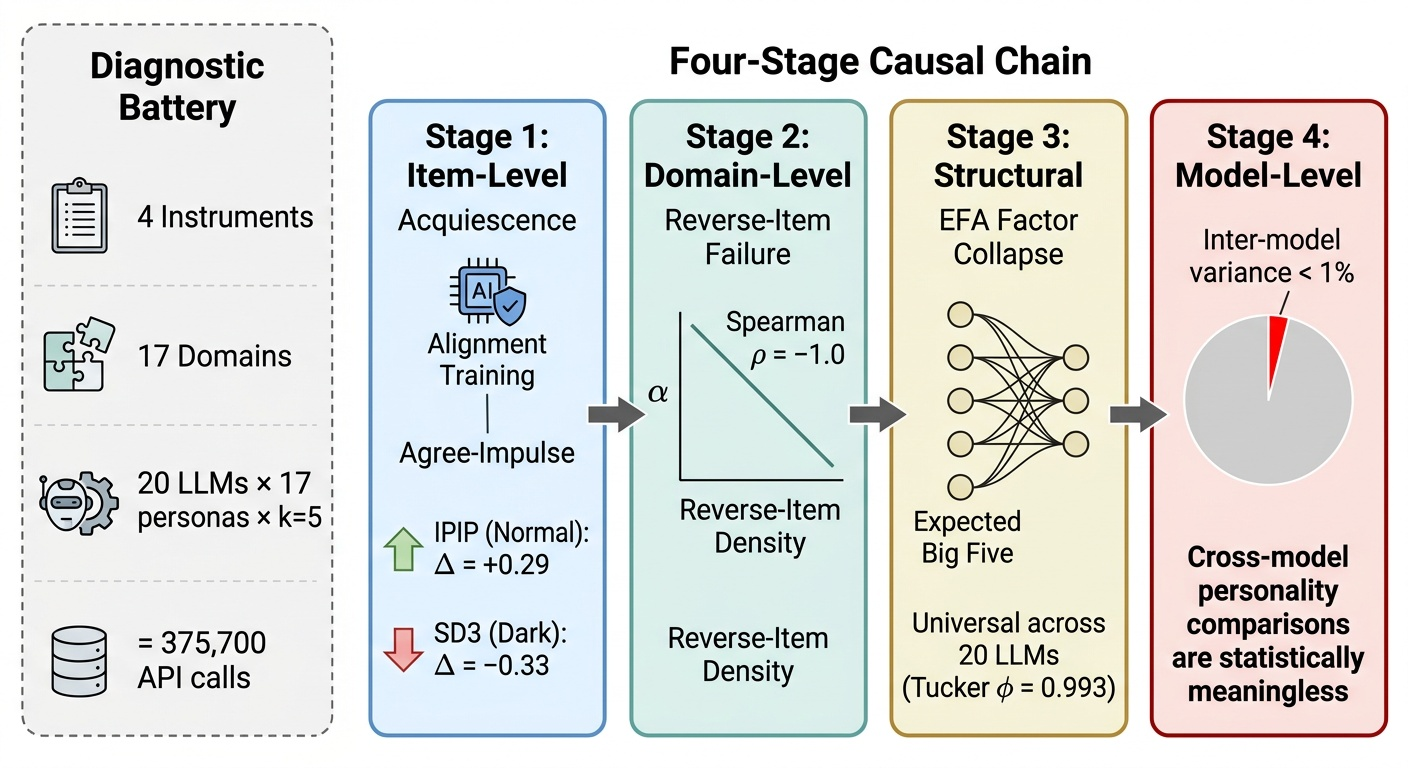
\includegraphics[width=\linewidth]{fig_causal_chain_overview.png}
  \caption{\textbf{From item-level acquiescence to model-level homogenisation: the causal chain that this paper documents.} Stage~1 (item-level acquiescence with directional asymmetry: IPIP $\Delta = +0.31$, SD3 $\Delta = -0.38$) $\to$ Stage~2 (Cronbach's $\alpha$ tracks reverse-item density at Spearman $\rho = -1.0$) $\to$ Stage~3 (EFA collapses 5 Big Five factors into 3 universally, Tucker's $\varphi = 0.993$) $\to$ Stage~4 (inter-model variance below $1\%$ of total Sum-of-Squares). The chain holds across 20 LLMs $\times$ 17 personas $\times$ 4 instruments $\times$ $k{=}5$ samples = 375{,}700 raw API calls.}
  \label{fig:causal_chain_overview}
\end{figure}

Our contributions are:
\begin{itemize}\setlength\itemsep{0pt}
  \item \textbf{The first multi-model, multi-instrument psychometric validation study on LLMs.} 20 models $\times$ 8 vendor families $\times$ 4 validated instruments $\times$ 17 personas $\times$ $k=5$ samples = 375{,}700 raw API calls, orders of magnitude larger than prior LLM-personality work and explicitly diagnostic rather than profiling.
  \item \textbf{A single-cause causal chain from item to model.} Item-level acquiescence $\rightarrow$ alpha tracks reverse density at $\rho=-1.0$ $\rightarrow$ EFA collapses five factors into three with Tucker's $\varphi=0.993$ $\rightarrow$ inter-model variance $<1\%$.
  \item \textbf{The directional-asymmetry framing} that unifies sycophancy~\citep{perez2023discovering,sharma2024sycophancy} and safety-driven rejection~\citep{bai2022constitutional} as two faces of one alignment artefact.
  \item \textbf{A persona stress test} that quantifies role compliance without measurement validity (PSD~$1.198$, $99.7\%$ nearest-centroid recovery, cross-scale coherence~$0.839$, Fwd/Rev coherence~$0.696$) and the resulting scope conditions on persona-conditioned multi-agent simulations.
  \item \textbf{Synthetic-baseline calibration} that rules out a ``trait $+$ style noise'' generative model.
  \item \textbf{An item-level plasticity map} of the alignment safety floor (visible-behaviour items shift up to $0.63$ under persona prompts; safety- and morality-anchored items do not move).
  \item \textbf{A methodological prescription} for future LLM-personality work: report internal consistency, factor structure, convergent validity, and measurement invariance before interpreting any score; establish invariance before cross-condition comparisons; adopt multi-temperature and multi-seed designs.
\end{itemize}

\noindent The six-check battery and the persona stress test that organise the rest of the paper are summarised schematically in Appendix~\ref{app:battery-schema} (Figure~\ref{fig:validation_battery_schema}).

\section{Related Work}
\label{sec:related}

\subsection{LLM personality profiling and silicon samples}
\label{sec:related-profiling}

The dominant strand of work on LLM personality administers a human inventory to one or more models and reports the resulting profile. \citet{miotto2023gpt3} kick off this line with the NEO-PI-R and a Schwartz values survey on GPT-3. \citet{serapio2025psychometric} formalise a psychometric framework for the IPIP-NEO on Google's PaLM family and report shapable Big Five profiles. \citet{jiang2023personallm} extend the same template to PersonaLLM. \citet{huang2023psychobench} consolidate thirteen scales into the PsychoBench suite. \citet{bodroza2024personality} run temporal-stability tests across several frontier models, and \citet{lee2025trait} release the TRAIT testset built explicitly around the Big Five. Adjacent work brings cognitive-psychology probes~\citep{binz2023psychology} and trait-descriptor recovery~\citep{suh2024rediscovering} to the same population.

A parallel literature converts these profiles into operational predictions. \citet{argyle2023one} propose that LLMs conditioned on demographic backstories can simulate human survey samples; \citet{horton2023homo} extends the proposal to economic experiments; \citet{aher2023using} replicate classic behavioural studies on simulated human cohorts; \citet{park2023generative} embed persona-conditioned LLMs in a small interactive society; \citet{ferreira2025matching} attempt to replicate EPQR-A population structure on GPT-simulated samples. The silicon-sample programme inherits whatever measurement error sits in the underlying personality scores: if the inventories do not measure traits on LLMs, the simulated survey responses cannot be trusted either~\citep{tjuatja2023response,salecha2024llm,larooij2025validation}.

A small but growing critical literature has begun to push back. \citet{salecha2024llm} document social-desirability bias on Big Five surveys. \citet{suhr2025challenging} challenge the validity of LLM personality tests at the Web Conference. \citet{pelet2025persistent} report instability across scale, reasoning, and conversation history. \citet{han2025personality} expose a dissociation between LLM self-reports and downstream behaviour, and \citet{mannekote2025roleplaying} extend the same dissociation to role-playing trust agents. \citet{xie2025aipsychobench} introduce a psychometric-difference benchmark, and~\citet{chen2025humanizing} survey the area. A parallel strand applies persona-conditioned LLMs as agents inside generative social simulations of opinion dynamics, debate, and polarisation~\citep{chuang2023simulating,cau2025language,chuang2025debate} or replicates psychometric population structures end-to-end~\citep{ferreira2025matching}; \citet{larooij2025validation} systematically review this literature and identify validation as the central unmet challenge --- existing simulations rely on face validity rather than measurement-grounded calibration. Common to almost all of this work is a single-instrument design, a single check (typically test-retest stability or Cronbach's $\alpha$), and a handful of models. The directional asymmetry of acquiescence between normal-personality and dark-trait inventories, the universality of the three-factor collapse under multi-instrument exploratory factor analysis, and the cross-model variance shrinkage to below one per cent of total sum of squares are, to our knowledge, not previously documented in a single audit. Our six-check battery plus persona stress test on twenty models and four instruments closes this gap and supplies the measurement-grounded calibration that downstream silicon-sample and persona-agent simulations need.

Our contribution is distinct from the most closely related audits. \citet{suhr2025challenging} establish that measurement invariance fails for BFI-2 on three GPT-family models; we extend this in four ways --- (i) we identify acquiescence as the common upstream mechanism rather than reporting each failure in isolation, (ii) we quantify its directional asymmetry across normal and dark-trait content, (iii) we show that even maximal persona steering does not repair the instruments, and (iv) we demonstrate universality across 20 models and 4 instruments rather than 3 models and 1. \citet{serapio2025psychometric} reach the opposite conclusion, that psychometrically valid personality measurement is possible; the discrepancy is methodological: their BFI-2 instrument carries only $\approx15\%$ reverse-keyed items (versus $29\%$ here), they sample deterministically at $T{=}0$, and they do not test reverse-item consistency --- the central failure mode our audit identifies. More broadly, sycophancy, social-desirability bias, and prompt sensitivity have each been documented as separate behavioural observations~\citep{perez2023discovering,sharma2024sycophancy,salecha2024llm}; our claim is structurally different --- a measurement-level verdict about their joint, quantifiable, and (under persona steering) non-repairable downstream damage to instrument validity.

\subsection{Response styles, acquiescence, and social desirability}
\label{sec:related-styles}

Human survey methodology has spent six decades cataloguing and controlling response styles. \citet{couch1960yeasayers} introduced acquiescence (``yea-saying'') as a personality variable; \citet{crowne1960social} developed the canonical social-desirability scale; and \citet{paulhus1991response} synthesised the field into a unified taxonomy. \citet{billiet2000modeling} model acquiescence as an explicit factor in structural-equation models of balanced item sets, and \citet{baumgartner2007modeling} document its cross-national footprint in marketing research. The standard countermeasure is reverse-keyed items: items written so that endorsement maps to the negative pole of the trait. Reverse-keyed items act both as a corrective on individual responses and as a diagnostic --- their inconsistency with forward items quantifies how much of the variance is response style rather than substance.

The diagnostic apparatus built around this idea is the same toolkit our audit imports wholesale. Cronbach's $\alpha$~\citep{cronbach1951coefficient} provides per-domain internal consistency; classical test theory~\citep{lord1968statistical} provides the underlying variance partition; exploratory factor analysis under the Kaiser eigenvalue criterion~\citep{kaiser1960application}, Horn's parallel analysis~\citep{horn1965parallel}, and varimax rotation~\citep{kaiser1958varimax} recovers latent structure; Tucker's coefficient of congruence~\citep{tucker1951method} quantifies replication; \citet{meredith1993measurement} formalised measurement invariance, and \citet{vandenberg2000review} compiled the operational checklist that organisational research now follows. Forced-choice and ipsative inventories built on item-response theory have been proposed as structural alternatives that bypass response styles entirely~\citep{brown2011forcedchoice,treaux2025forced}. Bootstrap inference~\citep{efron1979bootstrap} and Mahalanobis covariance distance~\citep{mahalanobis1936generalised} round out the statistical toolkit our audit uses.

Two limitations of the existing LLM literature stand out against this backdrop. First, the response-style toolkit has not been imported in coherent form: where reverse-keyed inconsistency is reported~\citep{acquiescence2025emnlp}, it is reported as a curiosity rather than as a quantitative diagnostic with a falsifiable structural signature. Second, the directional asymmetry between agree-pull on normal-personality items and reject-pull on dark-trait items has not been documented at the item level. We argue these are symptoms of the same alignment-driven mechanism, observable simultaneously through the same forward/reverse decomposition, and that this unification is precisely what closes the chain from item-level acquiescence to model-level homogenisation.

\subsection{Alignment, RLHF, and behavioural side effects}
\label{sec:related-alignment}

Almost every commercial LLM in our study has been trained with some combination of supervised instruction tuning~\citep{wei2022flan,ouyang2022training}, reinforcement learning from human or AI feedback~\citep{christiano2017deep,ouyang2022training,bai2022constitutional}, and direct preference optimisation~\citep{rafailov2023dpo}. The behavioural side effects of these regimens are increasingly well documented. \citet{perez2023discovering} use model-written evaluations to surface a wide spectrum of value-laden behaviours, including sycophancy and political bias. \citet{sharma2024sycophancy} characterise sycophancy as a robust failure mode that survives across multiple alignment recipes. \citet{kirk2023understanding} show that RLHF systematically reduces output diversity and homogenises generation distributions. \citet{zheng2024agreeableness} quantify agreeableness-driven sycophancy in role-playing contexts, and \citet{wang2024aligning} probe the limits of RLHF-based alignment. Survey-design probes corroborate this picture: \citet{tjuatja2023response} show that LLMs exhibit human-like response biases on survey items, and \citet{salecha2024llm} demonstrate alignment-shaped social-desirability bias on Big Five inventories.

What this strand has not yet done is connect these side effects to classical response-style theory and show that they produce a single mechanistically traceable failure of measurement validity across the standard psychometric checks. The closest precedent is the survey-design line~\citep{tjuatja2023response,dominguez2024questioning} and the recent self-report-versus-behaviour dissociation~\citep{han2025personality}, but neither closes the loop from item-level acquiescence to model-level variance collapse. We treat alignment-induced acquiescence and its directional inversion on dark-trait items as the unified mechanism that explains (i) the $\alpha$--reverse-density rank-1 inverse relationship, (ii) the universal three-factor collapse with Tucker's $\varphi=0.993$, (iii) inter-model variance below one per cent, (iv) the item-level plasticity dichotomy between visible-behaviour items and a safety floor, and (v) persona compliance without measurement validity. Reading personality scores off chat-tuned LLMs without first auditing the instrument therefore measures the alignment layer at least as much as it measures any putative trait~\citep{laverghetta2022predicting}.

% ----------------------------------------------------------------------
% Section 3: Methodology
% ----------------------------------------------------------------------

\section{Methodology}
\label{sec:method}

\begin{table}[t]
\centering
\small
\begin{tabular}{lrlrr}
\toprule
Instrument & Items & Format & Doms & Rev \\
\midrule
IPIP-NEO-120~\citep{johnson2014measuring}  & 120 & Likert-5 & 5 & 41 \\
SD3~\citep{jones2014introducing}     & 27  & Likert-5 & 3 & 5  \\
ZKPQ-50-CC~\citep{aluja2006cross}    & 50  & T / F    & 5 & 12 \\
EPQR-A~\citep{francis1992development}     & 24  & Y / N    & 4 & 5  \\
\midrule
\textbf{Total} & \textbf{221} & 3 formats & \textbf{17} & \textbf{63} \\
\bottomrule
\end{tabular}
\caption{The 221-item battery: 4 inventories, 3 response formats, 17 domains, 63 reverse-keyed items ($28.5\%$).}
\label{tab:battery}
\end{table}

\paragraph{Battery (Table~\ref{tab:battery}).} IPIP-NEO-120 covers the Big Five at the domain level; SD3 adds the three Dark Triad constructs; ZKPQ-50-CC adds Activity, Aggression-Hostility, Impulsive Sensation Seeking, Neuroticism-Anxiety, and Sociability in true/false format; EPQR-A adds Eysenck Psychoticism, Extraversion, Neuroticism, and a Lie scale in yes/no format. The multi-instrument design is required by the convergent-validity and cross-scale coherence checks: no single inventory provides the redundant cross-format measurements those tests need.

\paragraph{Models and protocol.} We query 20 instruction-tuned LLMs across 8 vendor families: Anthropic Claude-Opus-4.6 and Claude-Sonnet-4.6; OpenAI GPT-5.2 and GPT-5.5~\citep{openai2023gpt4}; Google Gemini-3-Pro / -Flash and Gemini-3.1-Pro / -Flash-Lite~\citep{gemini2024v15}; DeepSeek V3.2, V4-Flash, V4-Pro~\citep{deepseek2024v3}; Alibaba Qwen3-235B-A22B, Qwen3.5-122B-A10B, Qwen3.5-397B-A17B~\citep{qwen2024qwen25}; Zhipu GLM-4.6V, GLM-4.7, GLM-5.1~\citep{glm2024chatglm}; Moonshot Kimi-K2.5 and Kimi-K2.6~\citep{moonshot2025kimi}; and MiniMax-M2.7~\citep{minimax2025minimax01}. Each model is queried at $T{=}0.7$ with $k{=}5$ samples per (model, persona, item) cell. The 17 conditions are a Default no-persona instruction (``Please answer the following personality questionnaire honestly.'') plus all 16 MBTI personas administered as \texttt{"Respond as if you have <TYPE> personality."}. The completed corpus contains $20 \times 17 \times 221 = 75{,}140$ averaged item scores from $375{,}700$ raw API calls; $61$ refusals ($0.0162\%$, all under Default) are mean-imputed per item (Appendix~\ref{app:missing}).

\paragraph{Six validity checks.} (i)~\emph{Internal consistency}: Cronbach's $\alpha$~\citep{cronbach1951coefficient} per IPIP domain, treating the $17 \times 20 = 340$ (persona, model) cells as observations. (ii)~\emph{Factor structure}: EFA on the standardised $340 \times 17$ domain matrix with Kaiser~\citep{kaiser1960application} and parallel-analysis~\citep{horn1965parallel} retention, varimax rotation~\citep{kaiser1958varimax}, replicated leave-one-model-out (20 reruns), per-family (8), per-model (20); congruence reported by Tucker's $\varphi$~\citep{tucker1951method}. (iii)~\emph{Reverse-item consistency}: Pairwise Inconsistency Rate per (model, domain) and per-instrument forward-vs-reverse agree-rate gap $\Delta$. (iv)~\emph{Variance decomposition}: marginal (Type-III) SS partition over Model $+$ Domain $+$ Persona $+$ Item $+$ Residual, separately on Likert and binary composites (because the factors are non-orthogonal, marginal components need not sum to the total; Residual is the remainder). (v)~\emph{Convergent validity}: Pearson and Spearman across 20 model-level means for 8 pre-specified construct pairs. (vi)~\emph{Measurement invariance}: Pearson $r$ between each model's Default item vector and each of its 16 MBTI item vectors; strong-invariance threshold $r > 0.8$~\citep{vandenberg2000review,meredith1993measurement}.

\paragraph{Persona stress test and baselines.} Persona Separation Degree (PSD) is the normalised 17-d Euclidean distance from Default in z-space divided by $\sqrt{17}$. Nearest-centroid persona classification uses leave-one-model-out centroids in z-Euclidean, cosine, and Mahalanobis~\citep{mahalanobis1936generalised} metrics. Target adherence, sign-aligned cross-scale coherence, forward/reverse pair coherence, item-level plasticity, and a factorial main-effects model for the four MBTI axes complete the stress test. For calibration, three synthetic baselines on the IPIP structure --- Random, Pure Acquiescence, Trait+Acquiescence --- anchor floor and ceiling; aggregates carry bootstrap 95\% CIs~\citep{efron1979bootstrap}.

% ----------------------------------------------------------------------
% Section 4: Experiments and Results
% ----------------------------------------------------------------------

\section{Experiments and Results}
\label{sec:results}

\subsection{Internal consistency: $\alpha$ tracks reverse density at $\rho = -1.0$}
\label{sec:results-alpha}

\begin{table}[t]
\centering
\small
\begin{tabular}{lrrrrr}
\toprule
Domain & LLM~$\alpha$ & LLM~SD & Human~$\alpha$ & Gap & Rev.\,\% \\
\midrule
Neuroticism       & 0.813 & 0.035 & 0.90 & $-0.087$ & 17 \\
Extraversion      & 0.928 & 0.008 & 0.89 & $+0.038$ & 17 \\
Openness          & 0.189 & 0.160 & 0.87 & $-0.681$ & 25 \\
Agreeableness     & 0.069 & 0.311 & 0.88 & $-0.811$ & 71 \\
Conscientiousness & 0.535 & 0.113 & 0.90 & $-0.365$ & 25 \\
\bottomrule
\end{tabular}
\caption{Cronbach's $\alpha$ per IPIP Big Five domain, averaged across 20 LLMs. Human baseline from~\citet{johnson2014measuring}. The gap to the human baseline is monotonically increasing in reverse-keyed item percentage; the Spearman rank correlation between LLM $\alpha$ and reverse percentage across the 5 domains is exactly $-1.0$ ($p < 0.01$).}
\label{tab:alpha}
\end{table}

Cronbach's $\alpha$ per IPIP Big Five domain, averaged across the 20 models (Table~\ref{tab:alpha}), reveals a clean rank-1 inverse relationship with reverse-keyed item density: Extraversion (17\% reverse, $\alpha=0.928$), Neuroticism (17\%, $\alpha=0.813$), Conscientiousness (25\%, $\alpha=0.535$), Openness (25\%, $\alpha=0.189$), Agreeableness (71\%, $\alpha=0.069$). Spearman $\rho(\alpha, \text{reverse\%}) = -1.0$ ($p < 0.01$); Figure~\ref{fig:alpha_vs_reverse_density} plots the gradient. Notice that two domains (Extraversion and Neuroticism) actually equal or exceed the human baseline --- this is not evidence of strong personality measurement on LLMs but a side effect of low reverse-item density: items the model is willing to agree with all cohere because the agree-impulse drives them in the same direction. The inverse relationship is not an artefact of the five IPIP domains: across all 17 domains the Spearman correlation between raw-score $\alpha$ and reverse-item percentage is $\rho=-0.83$ ($p<0.001$; $\rho=-0.75$ on the 14 non-degenerate domains), and the IPIP-five $\rho=-1.0$ is simply the clean end of a general law. We emphasise that this raw-score $\alpha$ pattern is a \emph{diagnostic signature of acquiescence} (forward and reverse items endorsed alike, destroying raw-score consistency in proportion to reverse density), not a claim that the items are unreliable; \S\ref{sec:results-correction} confirms this directly by removing acquiescence and showing that the signature is removable while the structural failure is not.

\begin{figure}[t]
  \centering
  
\includegraphics[width=\linewidth]{fig_alpha_vs_reverse_density.png}
  \caption{Cronbach's $\alpha$ (mean across 20 LLMs) vs reverse-keyed item percentage per IPIP Big Five domain. The 5 domains line up exactly along an inverse trend (Spearman $\rho{=}{-}1.0$, $p<0.01$). Human baseline $\alpha \approx 0.88$ shown for reference. Reverse-keyed items reject the LLM data.}
  \label{fig:alpha_vs_reverse_density}
\end{figure}

\subsection{Item-level acquiescence with directional asymmetry}
\label{sec:results-acquiescence}

Decomposing every model's responses into forward and reverse agree-rates per instrument (Table~\ref{tab:fwd_rev_delta}) reveals two opposite signs of the same bias: IPIP-NEO-120 forward-vs-reverse $\Delta=+0.31$ (classic acquiescence on normal-personality items); SD3 $\Delta=-0.38$, ZKPQ-50-CC $\Delta=-0.34$, EPQR-A $\Delta=-0.08$ (social-desirability rejection on dark-trait or non-normative items). Aggregated across instruments the gap is near zero ($+0.03$), but at the item level the same response pattern simultaneously produces agreement on socially desirable content and refusal on socially undesirable content (Figure~\ref{fig:acquiescence_directional_asymmetry}). Overall PIR $= 0.468$ with bootstrap 95\% CI $[0.413, 0.531]$; per-model correlation between reverse-agree rate and PIR is $+0.63$ (models that acquiesce more are more inconsistent). Persona prompts reduce PIR substantially: Default PIR-agreement of $0.674$ vs MBTI mean of $0.834$ (paired $t=10.70$, $p<0.0001$; Appendix~\ref{app:persona}, Figure~\ref{fig:pir_default_vs_mbti}).

\begin{figure}[t]
  \centering
  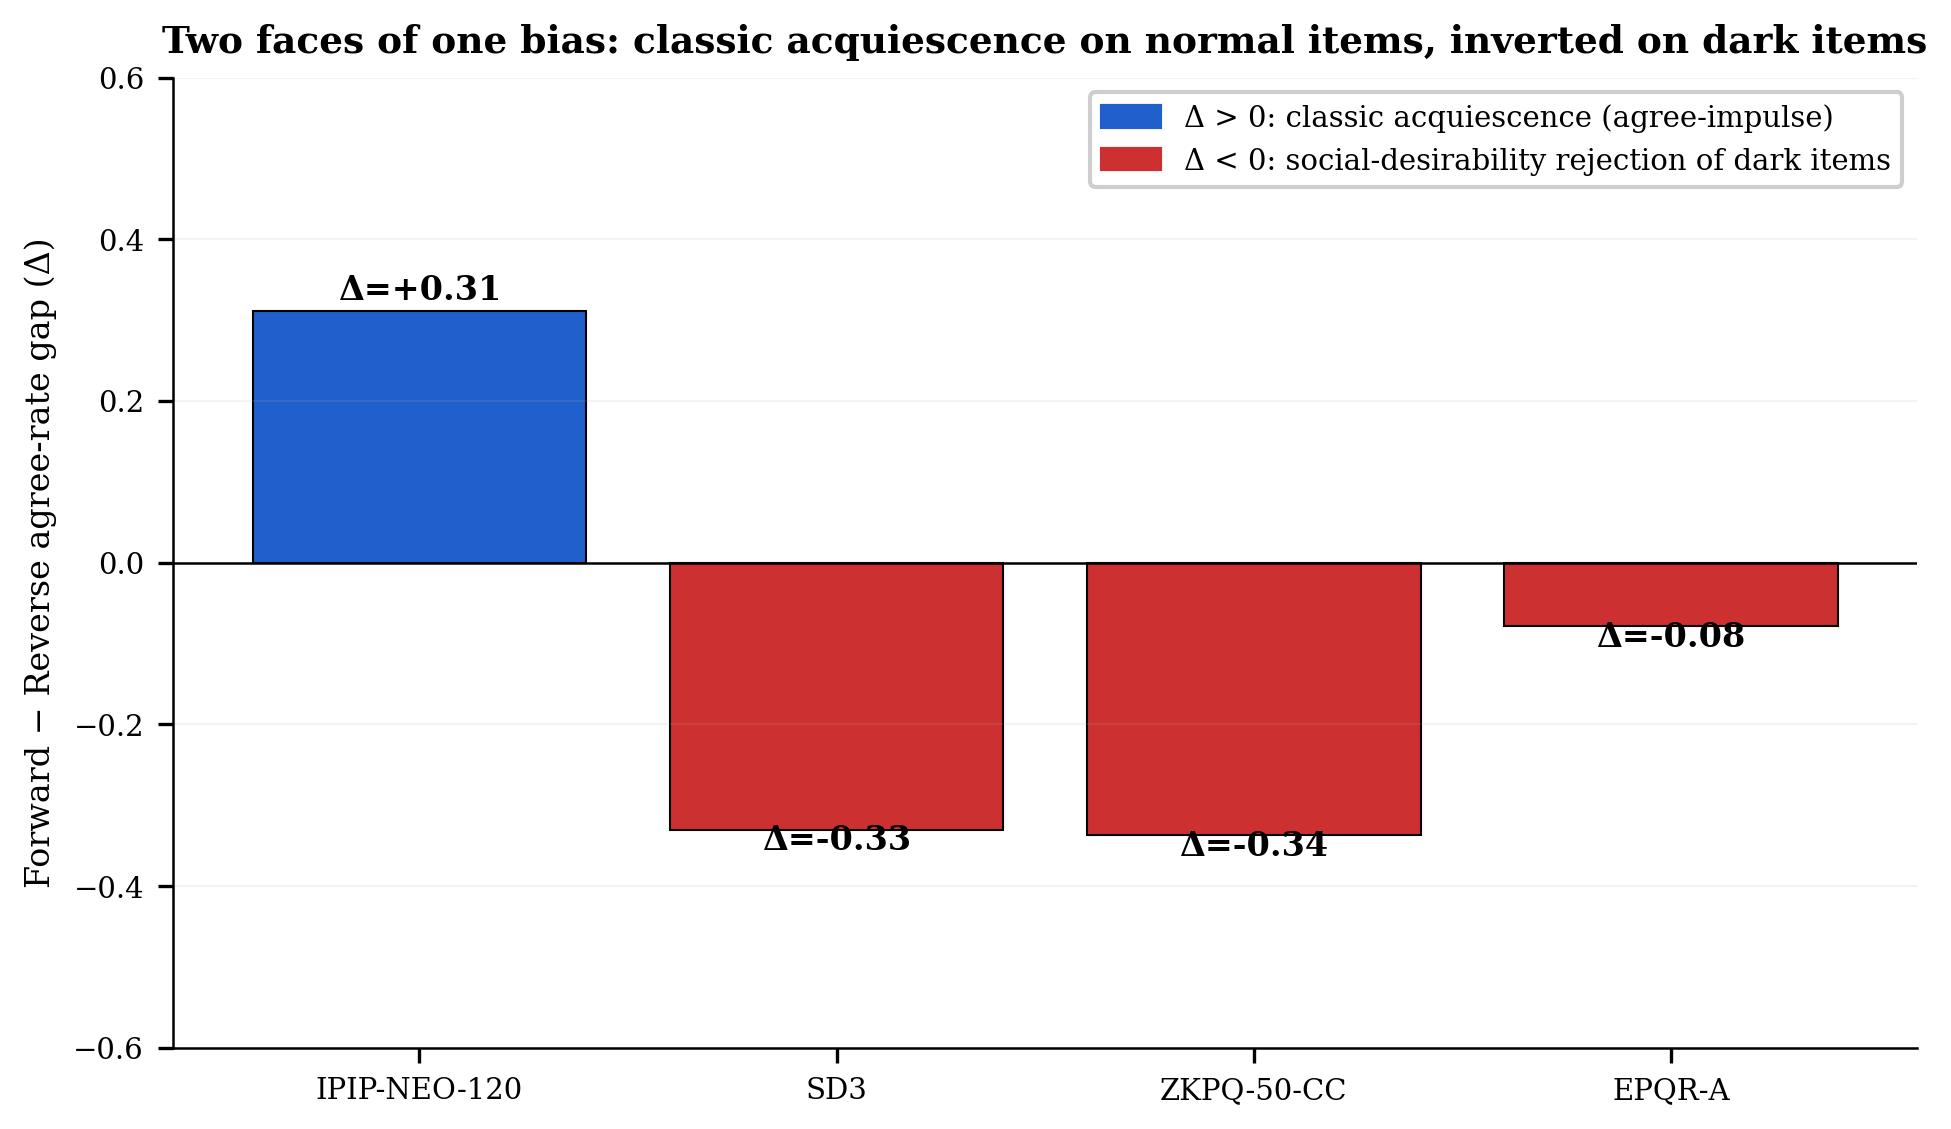
\includegraphics[width=\linewidth]{fig_acquiescence_directional_asymmetry.png}
  \caption{Forward-minus-reverse agree-rate gap per instrument, averaged across 20 LLMs. Positive bar (IPIP) is classic acquiescence; negative bars (SD3, ZKPQ, EPQR-A) are social-desirability rejection. Two faces of the same alignment-driven agree-impulse.}
  \label{fig:acquiescence_directional_asymmetry}
\end{figure}

\begin{table}[t]
\centering
\small
\begin{tabular}{lccc}
\toprule
Instrument & Fwd agree & Rev agree & $\Delta$ (Fwd$-$Rev) \\
\midrule
IPIP-NEO-120 & 0.67 & 0.35 & $+0.31$ \\
SD3          & 0.32 & 0.70 & $-0.38$ \\
ZKPQ-50-CC   & 0.12 & 0.45 & $-0.34$ \\
EPQR-A       & 0.08 & 0.16 & $-0.08$ \\
\midrule
Overall      & 0.42 & 0.39 & $+0.03$ \\
\bottomrule
\end{tabular}
\caption{Forward (Fwd) and reverse (Rev) item agreement rates and their gap $\Delta$, Default condition, mean over 20 models (agree $=$ Likert $\geq3$ or binary True/Yes). Positive $\Delta$ on IPIP is classic acquiescence; negative $\Delta$ on the dark/non-normative instruments is social-desirability rejection. Per-model values in \texttt{results/table4\_fwd\_rev\_delta.csv}.}
\label{tab:fwd_rev_delta}
\end{table}

\subsection{Factor structure: 5 expected, 3 observed, universally}
\label{sec:results-efa}

Both Kaiser ($\lambda > 1$) and parallel analysis retain exactly \textbf{3 factors} on the $340 \times 17$ matrix, against the expected 5 from Big Five theory (eigenvalues $\lambda_1 = 6.97, \lambda_2 = 4.33, \lambda_3 = 3.07$; first three factors explain 86--90\% of variance). The varimax loadings (Figure~\ref{fig:efa_loadings_heatmap}, full numerical table in Appendix~\ref{app:persona}, Table~\ref{tab:efa-loadings}) show that (i)~Extraversion-flavoured constructs --- IPIP Extraversion, ZKPQ Activity and Sociability, EPQR Extraversion, SD3 Narcissism --- collapse into a single F1; (ii)~Neuroticism merges with (inverted) Agreeableness and Machiavellianism into F2; and (iii)~Conscientiousness, EPQR Lie, and (inverted) ZKPQ Impulsive Sensation Seeking and EPQR Psychoticism load on F3. The collapse is universal: 20 leave-one-model-out reruns all return exactly 3 Kaiser factors (first-eigenvalue range 6.94--7.02; Tucker's $\varphi = 0.993$); 8 per-family reruns and 20 per-model reruns all return exactly 3 Kaiser factors (Appendix~\ref{app:persona}, Figure~\ref{fig:efa_loo_robustness}).

\begin{figure}[t]
  \centering
  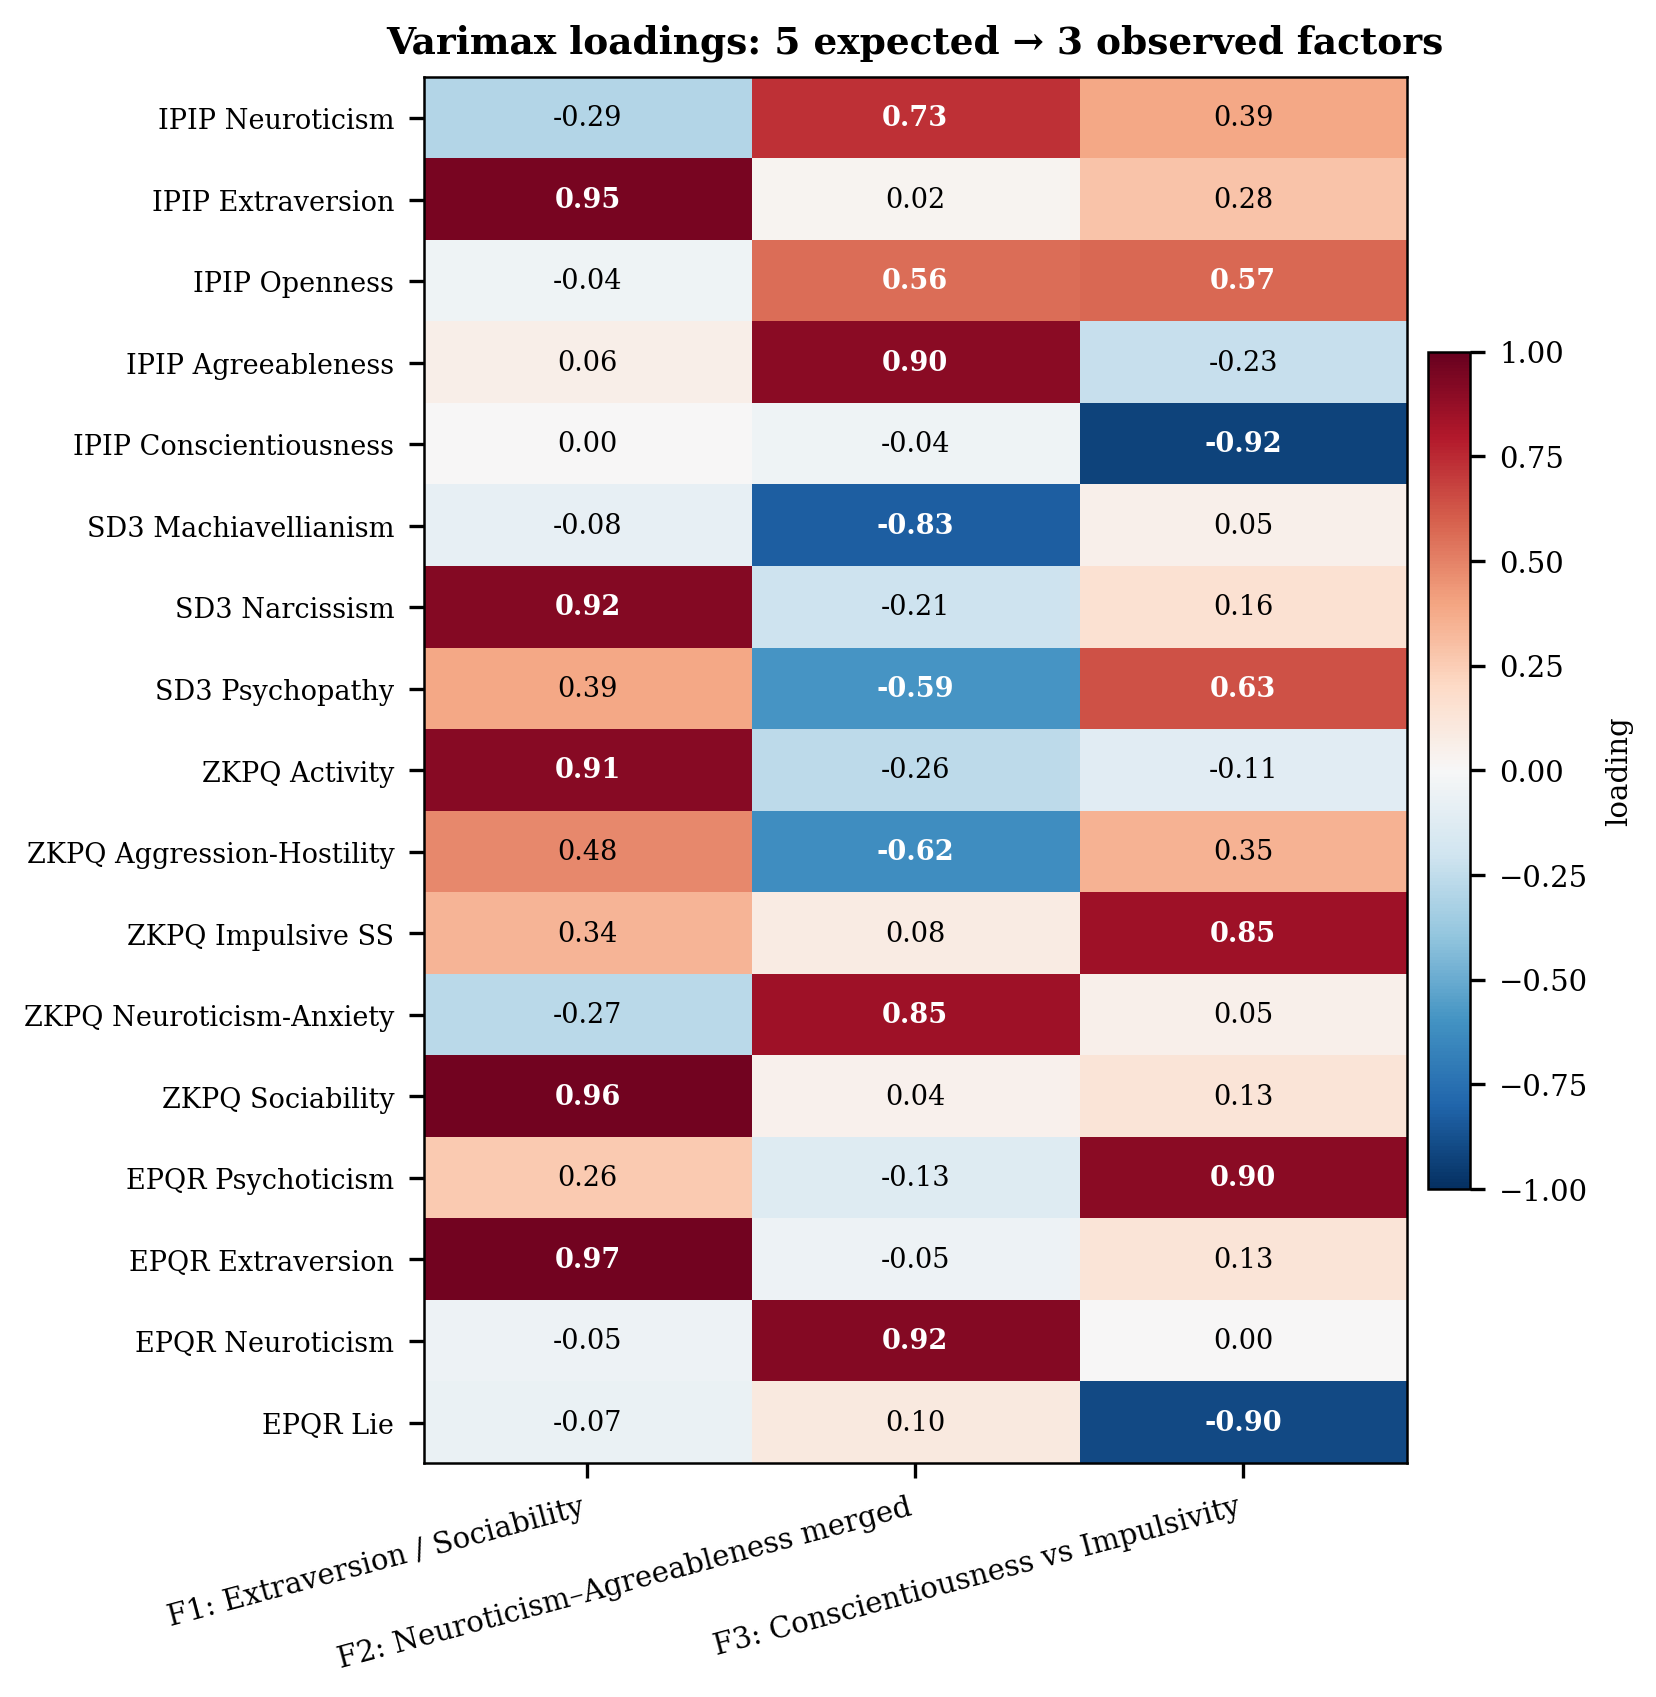
\includegraphics[width=\linewidth]{fig_efa_loadings_heatmap.png}
  \caption{Varimax-rotated factor loadings on the standardised 17-domain matrix ($n=340$). The expected 5-factor Big Five collapses into 3: Extraversion/Sociability, a fused Neuroticism-Agreeableness, and Conscientiousness vs Impulsivity.}
  \label{fig:efa_loadings_heatmap}
\end{figure}

\subsection{Acquiescence correction: symptom versus structure}
\label{sec:results-correction}

A reader may worry that the low raw-score $\alpha$ in reverse-heavy domains (\S\ref{sec:results-alpha}) is merely an artefact of computing $\alpha$ on un-reverse-scored items, rather than evidence of acquiescence. We test this directly in two steps. First, reverse-scoring the reverse-keyed items before computing $\alpha$ restores high $\alpha$ on every IPIP domain (mean $0.94$ versus $0.51$ on raw scores), confirming that the $\alpha$-versus-reverse-density pattern of Figure~\ref{fig:alpha_vs_reverse_density} is a \emph{diagnostic signature of acquiescence} (forward and reverse items endorsed alike) rather than a claim that the items are unreliable. Second, and more decisively, we apply the textbook statistical correction for acquiescence --- within-respondent mean-centering across all items~\citep{couch1960yeasayers} --- and re-run the EFA on the 17-domain matrix. The correction does \emph{not} recover the Big Five: the structure still yields three factors under both the Kaiser criterion and parallel analysis, with the eigenvalue profile essentially unchanged (top three $6.97/4.33/3.07 \to 7.00/3.73/3.46$; the fourth eigenvalue remains below $1$ in both cases). If a coherent five-factor structure were merely masked by acquiescence, removing it should reveal more factors; it does not. Two conclusions follow. The surface symptom (raw-score $\alpha$ tracking reverse density) and the structural verdict (five$\to$three collapse) are decoupled: the former is removable by reverse-scoring, the latter is not removable by the standard correction. And because high $\alpha$ after correction can reflect shared method variance rather than a recovered trait, $\alpha$ alone is not evidence of validity~\citep{cronbach1951coefficient}; the factor-structural collapse is the load-bearing result. This is consistent with the synthetic-baseline calibration below: the data resemble acquiescence-with-no-trait, not trait-plus-acquiescence.

\subsection{Model-level convergence: inter-model variance below 1\%}
\label{sec:results-variance}

\begin{table}[t]
\centering
\small
\begin{tabular}{lrr}
\toprule
Source & Likert (\%) & Binary (\%) \\
\midrule
\textbf{Model}    & \textbf{0.35} & \textbf{0.51} \\
Domain   & 23.93 & 5.27  \\
Persona  & 4.09  & 14.06 \\
Item     & 36.13 & 14.81 \\
Residual & 35.51 & 65.35 \\
\bottomrule
\end{tabular}
\caption{Marginal variance decomposition (\% of total Sum-of-Squares) into Model + Domain + Persona + Item + Residual terms, computed separately for the Likert (IPIP+SD3) and Binary (ZKPQ+EPQR) composites. Marginal components need not sum to 100\%. Inter-model variance is below 1\% on both composites (and remains below 2\% even under a sequential Type-I partition entering Model first).}
\label{tab:variance}
\end{table}

Marginal variance decomposition (Table~\ref{tab:variance}; Appendix~\ref{app:persona}, Figure~\ref{fig:variance_decomposition_likert_binary}) shows that inter-model variance accounts for $0.35\%$ of total Sum-of-Squares on the Likert composite and $0.51\%$ on the binary composite (a marginal/Type-III partition; the headline is robust, staying below 2\% even under a sequential Type-I partition that enters Model first). After accounting for the inventory's own structure (Domain), the prompted persona (Persona), and per-item variation (Item), almost nothing is left for the model. The question ``which LLM is more conscientious?'' is, at the resolution of these instruments, statistically meaningless --- cross-model comparisons are at best ranking models on residual noise.

\subsection{Convergent validity and calibration against synthetic baselines}
\label{sec:results-convergent}

Across the 20 model-level means we test 8 pre-specified construct pairs (Appendix~\ref{app:dif}, Table~\ref{tab:convergent}). Sign-match is $7/8$; the single failure is Extraversion $\times$ ZKPQ Sociability ($r_p = -0.10$, $p = 0.670$). Strongest convergence: Agreeableness $\times$ Psychopathy ($r_p = -0.81$), Conscientiousness $\times$ Psychopathy ($r_p = -0.73$), Agreeableness $\times$ Machiavellianism ($r_p = -0.71$). DIF across Western and Chinese vendor families is non-significant in every domain (all $p > 0.16$, max $|d| = 0.42$). To distinguish ``trait $+$ noise'' from ``no trait at all'', three synthetic baselines on the same IPIP structure (Appendix~\ref{app:dif}, Table~\ref{tab:synthetic}, Figure~\ref{fig:alpha_synthetic_baseline_calibration}): Random uniform and Pure Acquiescence both yield $\alpha \approx 0$; Trait+Acquiescence (genuine 5-factor latent structure plus acquiescence offset) recovers $\alpha > 0.99$ on every domain. LLM observed $\alpha$ sits close to Random / Pure-Acquiescence on the high-reverse-density domains (Agreeableness $0.07$, Openness $0.19$) and only approaches the human band on low-reverse-density domains where acquiescence inflation cannot be detected (Extraversion $0.93$, Neuroticism $0.81$). Pure acquiescence with no underlying trait is a quantitatively better generative model of the LLM data than ``trait with acquiescence on top.''

\subsection{Persona stress test: compliance without validity}
\label{sec:results-persona}

A persona stress test rules out the rescue that personality emerges only when the model is asked to play a character. MBTI prompts move profiles by more than one SD per dimension (mean PSD $= 1.198$, per-model range $0.996$--$1.384$, max $1.67$; Appendix~\ref{app:persona}, Figure~\ref{fig:persona_separation_degree}). Nearest-centroid persona classification recovers \textbf{319 / 320} pairs in z-Euclidean ($99.7\%$; Figure~\ref{fig:persona_fidelity_confusion_heatmap}); the single failure is DeepSeek-V3.2 ESFP $\to$ ENTP. Likert-only reaches $100\%$, cosine $99.7\%$, Mahalanobis $98.4\%$. Empirical target adherence averages $0.838$; theoretical-target adherence averages only $0.557$ --- LLMs reproduce an empirical persona pattern that diverges from the textbook MBTI description.

But persona compliance is not measurement validity. Three statistics fail simultaneously. \textbf{Measurement invariance} (Pearson $r$ between each model's Default vector and each MBTI vector) averages $r = 0.461$ across 320 pairs, with $0/320$ crossing $r > 0.8$. \textbf{Cross-scale coherence} of persona-induced shifts across instruments measuring the same construct is $0.839$ (95\% CI $[0.815, 0.862]$) --- below the $0.997$ nearest-centroid fidelity. \textbf{Forward/reverse pair coherence} is only $0.696$ ($0.737$ EPQR-A, $0.727$ ZKPQ, $0.685$ IPIP, $0.657$ SD3); on ${\approx}1/3$ of Fwd/Rev pairs the persona shift fails directional sanity. The factorial model also leaks across axes: EPQR Lie loads on J/P ($\beta = 0.78$); SD3 Narcissism loads on E/I ($\beta = 0.94$).

Item-level plasticity (Figure~\ref{fig:item_plasticity_distribution}) shows a sharp dichotomy: most-plastic items shift up to $0.63$ of scale range (EPQR ``Do you sometimes talk about things you know nothing about?'' $0.632$); most-locked items do not move (EPQR ``Do you enjoy hurting people you love?'' $0.000$; ``Take advantage of others'' $0.056$). The plasticity floor is the alignment safety filter, not the persona's plausible behaviour. Default-condition within-sample SD ($0.205$ Likert) exceeds every MBTI persona ($0.081$--$0.118$): persona prompts \emph{stabilise} responses (Appendix~\ref{app:wsc}).

% ----------------------------------------------------------------------
% Section 5: Conclusion
% ----------------------------------------------------------------------

\section{Discussion: Implications for {LLM-Based} Social Simulation}
\label{sec:conclusion}

A single alignment-induced acquiescence with a directional asymmetry ($\Delta = +0.29$ on normal items; $\Delta = -0.33$ on dark-trait items) explains why every standard psychometric check fails: $\alpha$ tracks reverse density at Spearman $\rho = -1.0$; EFA collapses 5 Big Five factors into 3 universally (Tucker's $\varphi = 0.993$); inter-model variance falls below $1\%$; and $0/320$ $(model, persona)$ pairs cross the strong-invariance threshold. Persona prompts are $99.7\%$ recoverable but yield only $0.839$ cross-scale and $0.696$ Fwd/Rev coherence --- compliance, not validity. Calibration places LLM data closer to ``no trait'' than to ``trait $+$ style''.

These findings impose scope conditions on the silicon-sample~\citep{argyle2023one,horton2023homo,ferreira2025matching} and persona-conditioned multi-agent simulation~\citep{chuang2023simulating,cau2025language,chuang2025debate,park2023generative} programmes. Persona prompts produce coarse, recoverable behavioural contrast --- $99.7\%$ of (model, persona) cells land in the right MBTI bin --- enough to differentiate ``agent A'' from ``agent B'' and to drive demographic stratification in silicon-sample surveys. They do \emph{not} produce a trait-grounded measurement substrate: persona shifts disagree across instruments measuring the same construct ($0.839$ coherence), reverse-keyed pairs fail directional sanity in ${\approx}1/3$ of cases, and the 3-factor collapse persists inside every persona condition.

Three consequences follow. (1)~Simulations whose conclusions depend on \emph{fine-grained psychological mechanisms} --- factor-pure trait differences, trait-mediated causal chains, or interactions between Big Five facets --- inherit the 3-factor collapse and cannot recover the structure they assume. (2)~Simulations of \emph{extreme opinions, conflict dynamics, or polarisation}~\citep{chuang2025debate,cau2025language} run against the alignment safety floor: dark- and morality-anchored items have plasticity ${\approx}0$ across all 320 cells, so a persona-conditioned agent systematically under-expresses the very content that drives polarisation in human populations. (3)~The implicit ISTJ-like Default (8/20 models nearest ISTJ under leave-one-model-out classification, 12/20 ISTJ-like by empirical MBTI-axis projection; Appendix~\ref{app:persona}, Figure~\ref{fig:default_persona_classification}) injects a structured, cautious, non-confrontational role into every comparison --- ``no-persona'' is not neutral. The methodological prescription is direct: any LLM-personality claim should report internal consistency, factor structure, convergent validity, and measurement invariance before any score is interpreted; multi-temperature, multi-seed designs are necessary; and the choice between ``coarse persona contrast'' and ``trait-grounded mechanism'' should be made explicit at study design time. Reading personality off chat-tuned LLMs without auditing the instrument measures the alignment layer, not the model.

\paragraph{Future directions.} Because self-report questionnaires are not a valid measurement substrate for current LLMs, we point to four alternatives: (i) \emph{behavioural validation}, inferring traits from downstream choices or interactive tasks rather than self-report~\citep{han2025personality,mannekote2025roleplaying}; (ii) \emph{forced-choice / ipsative} formats that structurally bypass acquiescence by forcing trade-offs between equally desirable options~\citep{brown2011forcedchoice,treaux2025forced}; (iii) \emph{item-response-theory} models that separate trait from response-style parameters; and (iv) \emph{behavioural signatures} (consistency patterns, refusal profiles) invariant to prompt framing. To support replication we will release the six-check pipeline and the 375{,}700-response dataset.

% ----------------------------------------------------------------------
% Limitations
% ----------------------------------------------------------------------

\section*{Limitations}
\label{sec:limitations}

The study uses closed-weight commercial APIs only; alignment is diagnosed by mechanism rather than direct intervention against base / pre-RLHF baselines. We therefore cannot distinguish whether the shared acquiescent response style originates from alignment, from pre-training data, or from their interaction, and our causal language is correspondingly circumspect; a preliminary base/instruct comparison (Qwen3-0.6B, $k{=}1$) gives an overall reverse-item agree rate of $0.70$ (base) versus $0.77$ (instruct) --- both variants are highly acquiescent and instruction tuning shifts the rate only modestly --- but a single small model pair is insufficient to localise the source. Instruments and prompts are English; forced-choice, ipsative, behavioural-elicitation, and IRT-fitted alternatives are untested. Temperature is fixed at $0.7$ with $k{=}5$; multi-temperature and multi-seed designs are recommended but not run here. The persona stress test uses only the 16 MBTI types, and the implicit ISTJ-like Default may shift under alternative no-persona phrasings. Our scope conditions on LLM-based social simulation apply at the level of the underlying self-report measurement substrate: we do not evaluate behavioural-trace simulations~\citep{park2023generative} or simulations whose outputs are anchored to verifiable external data rather than self-report scores. Conclusions concern currently deployed instruction-tuned chat models and make no claim about future architectures.

% ----------------------------------------------------------------------
% Ethics Statement
% ----------------------------------------------------------------------

\section*{Ethics Statement}
\label{sec:ethics}

The study involves no human subjects. All data are LLM API responses to published validated inventories used under their original research-use terms. The work is motivated by a public-good concern that unsupported personality-trait claims about LLMs propagate into alignment, hiring, and public-opinion applications. All 61 refusals are reported transparently (Appendix~\ref{app:missing}); no attempt was made to evade safety filters or retry refused calls. Anonymised data and code release are deferred to post-acceptance.

% ----------------------------------------------------------------------
% Bibliography
% ----------------------------------------------------------------------

\bibliography{refs}

\clearpage
\appendix

% ----------------------------------------------------------------------
% Appendix A: Persona Steering Supplement
% ----------------------------------------------------------------------

\section{Persona Steering Supplement}
\label{app:persona}

\begin{figure*}[t]
  \centering
  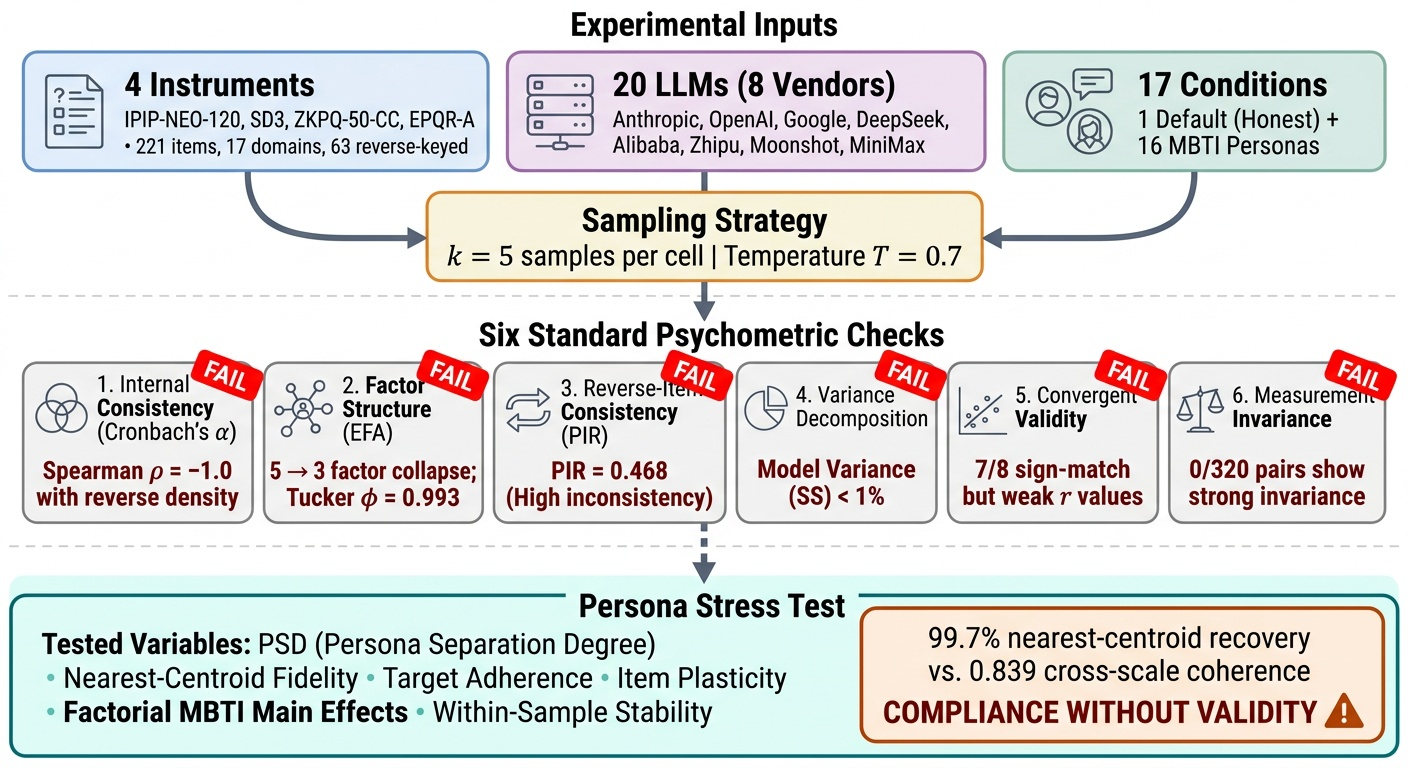
\includegraphics[width=0.95\linewidth]{fig_validation_battery_schema.png}
  \caption{Schematic of the six-check psychometric validation battery plus persona stress test applied to 20 LLMs on the 221-item battery. Each check displays a FAIL badge with its diagnostic outcome.}
  \label{fig:validation_battery_schema}
\end{figure*}
\label{app:battery-schema}

\subsection{Persona fidelity and item plasticity}

Figure~\ref{fig:persona_fidelity_confusion_heatmap} reports the 16$\times$16 confusion matrix of nearest-centroid persona classification with LOO centroids; only one off-diagonal cell. Figure~\ref{fig:item_plasticity_distribution} shows the per-item plasticity distribution across content categories.

\begin{figure}[t]
  \centering
  
\includegraphics[width=\linewidth]{fig_persona_fidelity_confusion_heatmap.png}
  \caption{Nearest-centroid persona classification (z-Euclidean, LOO): 319/320 (model, persona) pairs recovered; single confusion is DeepSeek-V3.2 ESFP $\to$ ENTP.}
  \label{fig:persona_fidelity_confusion_heatmap}
\end{figure}

\begin{figure}[t]
  \centering
  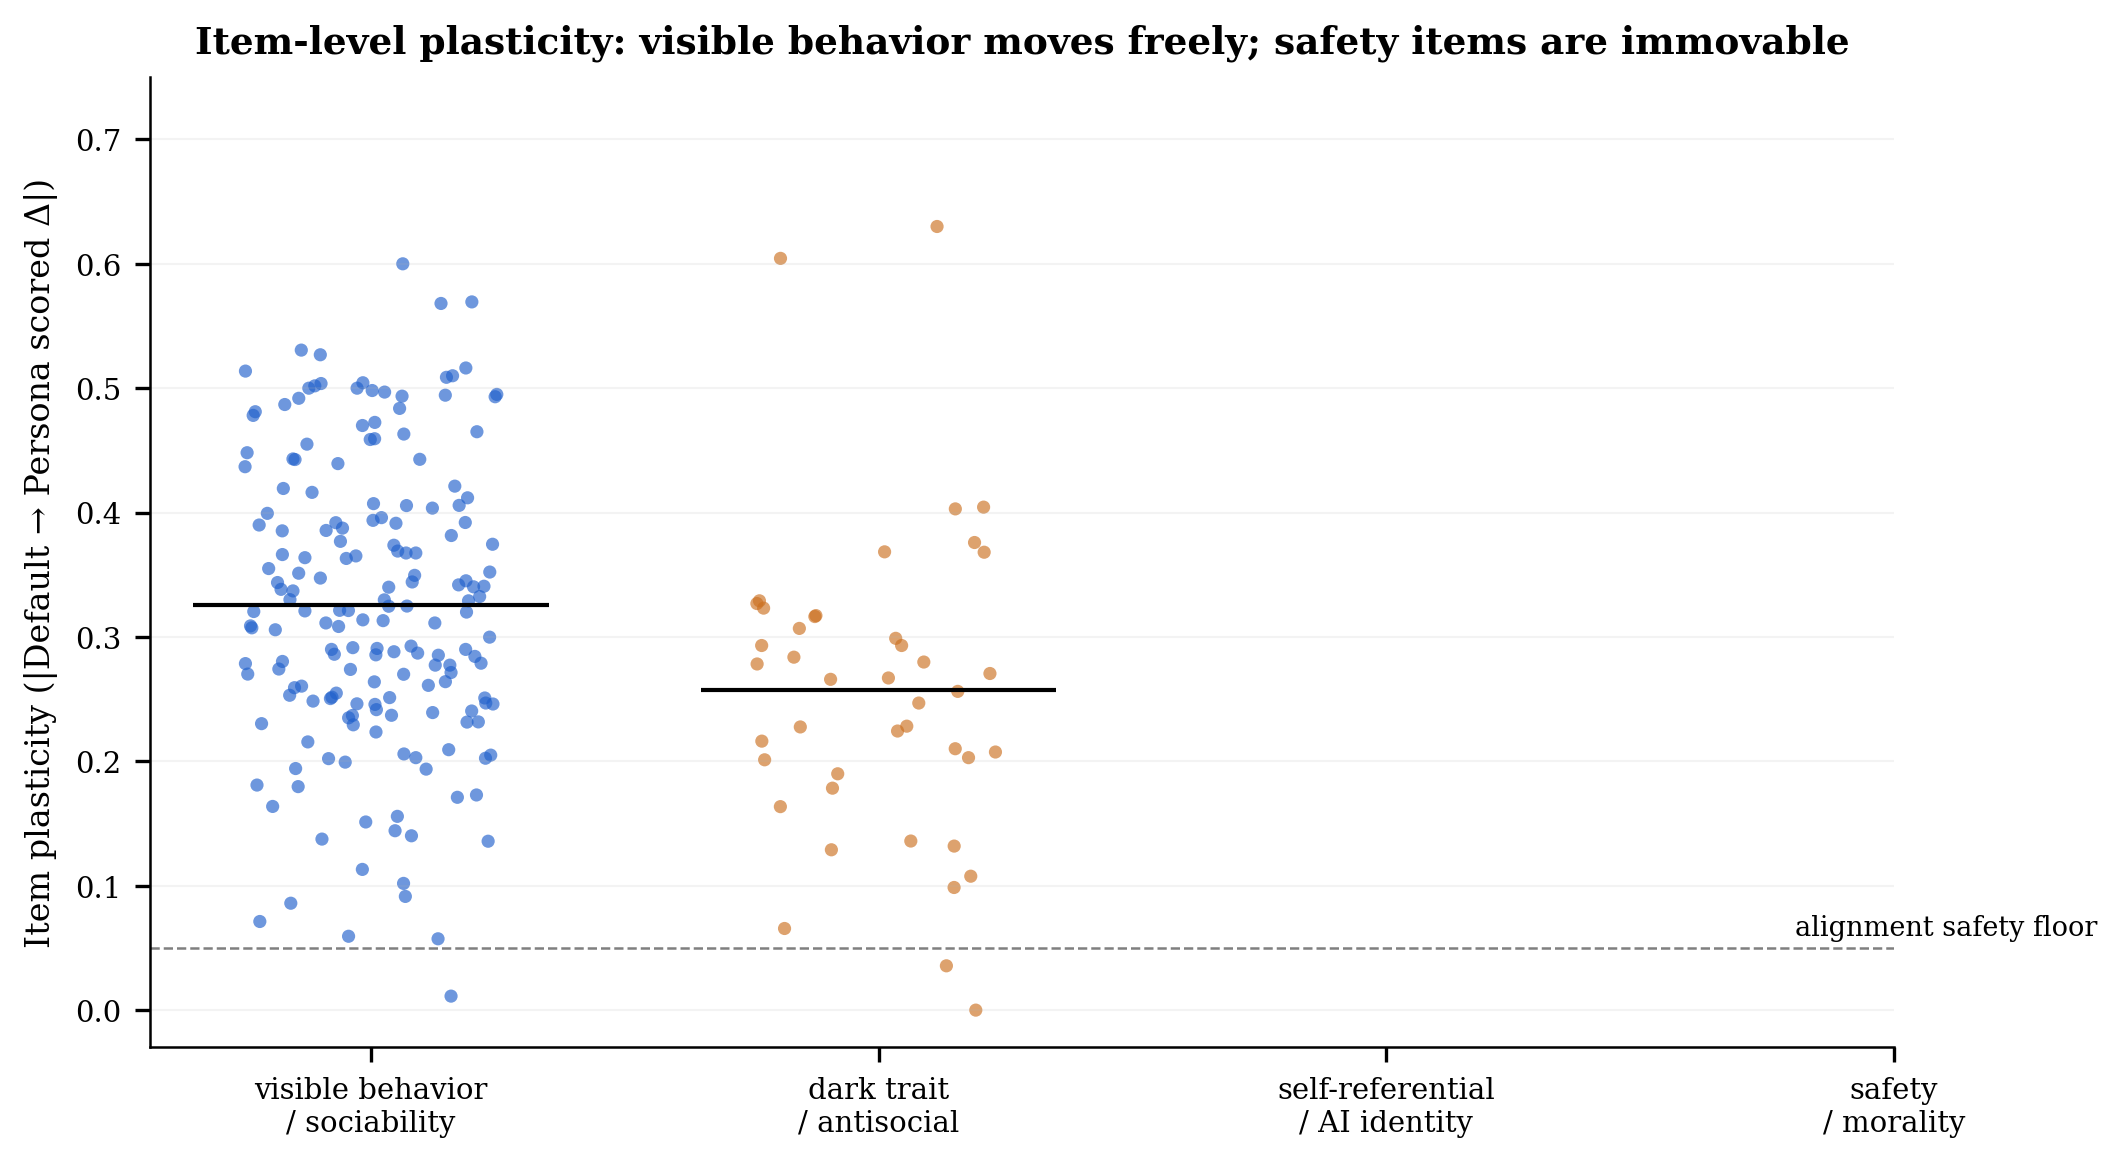
\includegraphics[width=\linewidth]{fig_item_plasticity_distribution.png}
  \caption{Item-level plasticity (mean absolute Default-vs-persona scored shift, normalised by scale range) across 221 items, by content category. Visible-behaviour items reach 0.6 plasticity; safety / morality items are pinned at 0.}
  \label{fig:item_plasticity_distribution}
\end{figure}

\subsection{Per-model Persona Separation Degree and within-sample stability}

Figure~\ref{fig:persona_separation_degree} reports the per-model PSD across the 16 MBTI personas. Mean PSD across all models is $1.198$; Gemini-3-Pro is the most steerable at $1.384$ and MiniMax-M2.7 the least at $0.996$. The peak persona is overwhelmingly ENTP or ESTP --- the two MBTI types that push hardest against the implicit ISTJ-like Default baseline.

\begin{figure}[t]
  \centering
  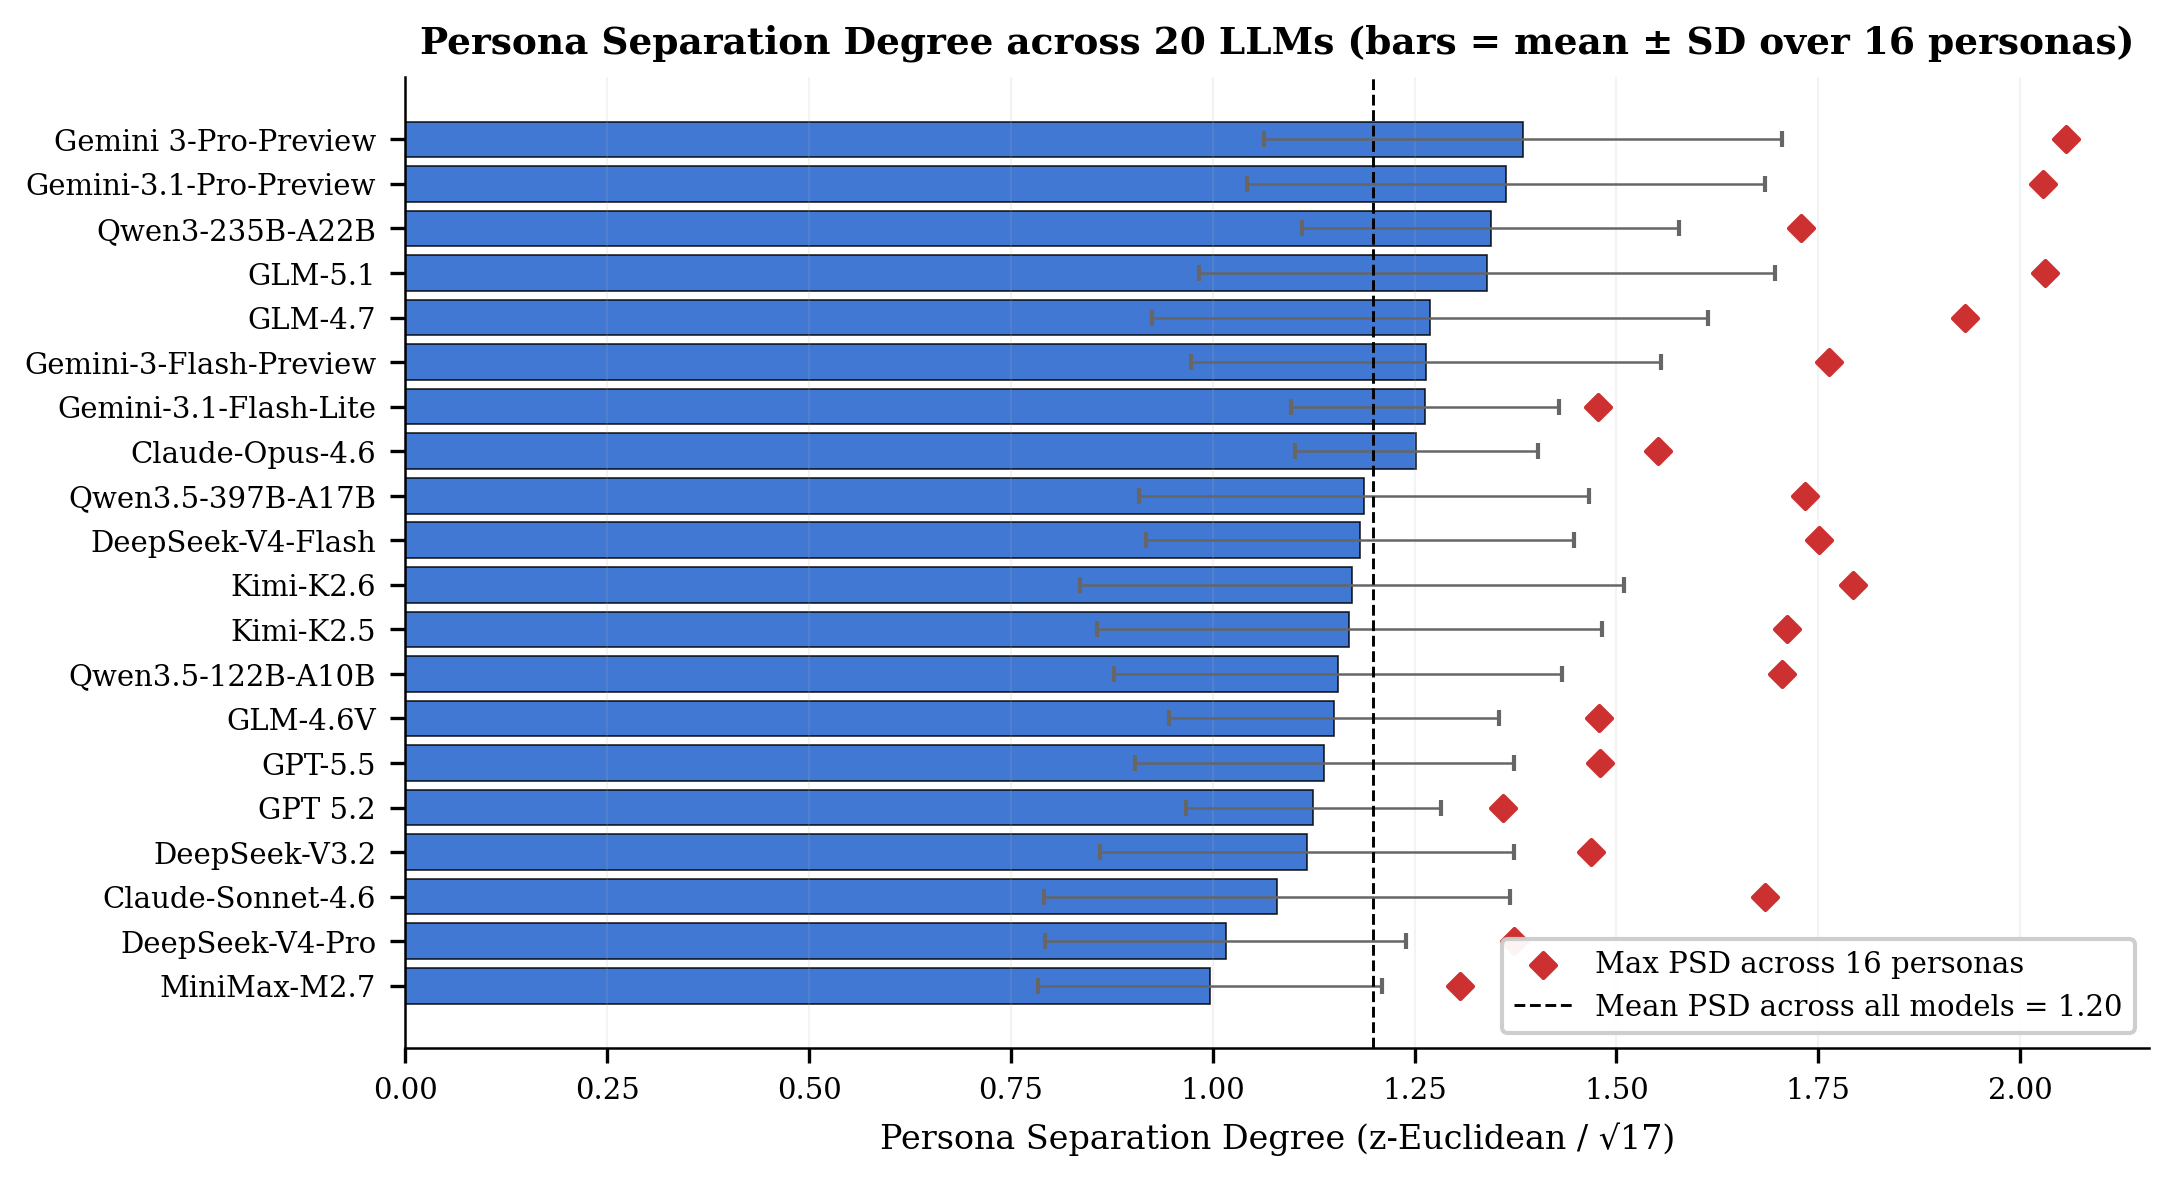
\includegraphics[width=\linewidth]{fig_persona_separation_degree.png}
  \caption{Persona Separation Degree (mean across 16 MBTI personas, bars; max, diamonds; SD as error bars) per model.}
  \label{fig:persona_separation_degree}
\end{figure}

\subsection{Measurement invariance distribution}

Figure~\ref{fig:measurement_invariance_histogram} shows the histogram of Pearson $r$ between Default and each MBTI item vector across the 320 (model, persona) pairs. Mean $r = 0.461$; the strong-invariance threshold $r > 0.8$ is crossed by 0/320 pairs.

\begin{figure}[t]
  \centering
  
\includegraphics[width=\linewidth]{fig_measurement_invariance_histogram.png}
  \caption{Default-vs-MBTI item-vector Pearson $r$ across 320 (model, persona) pairs. 0/320 pairs are above the strong-invariance threshold.}
  \label{fig:measurement_invariance_histogram}
\end{figure}

\subsection{Cross-scale coherence and target adherence}

Figure~\ref{fig:cross_scale_coherence_by_construct} reports sign-aligned cross-scale coherence by construct (Extraversion $0.898$, Neuroticism $0.868$, Conscientiousness-vs-Disinhibition $0.800$, Agreeableness-vs-Antagonism $0.790$; overall $0.839$ [bootstrap 95\% CI $0.815$, $0.862$]; sign-match $0.788$). The dashed reference at $0.997$ marks nearest-centroid persona recovery, exposing the compliance / validity gap.

\begin{figure}[t]
  \centering
  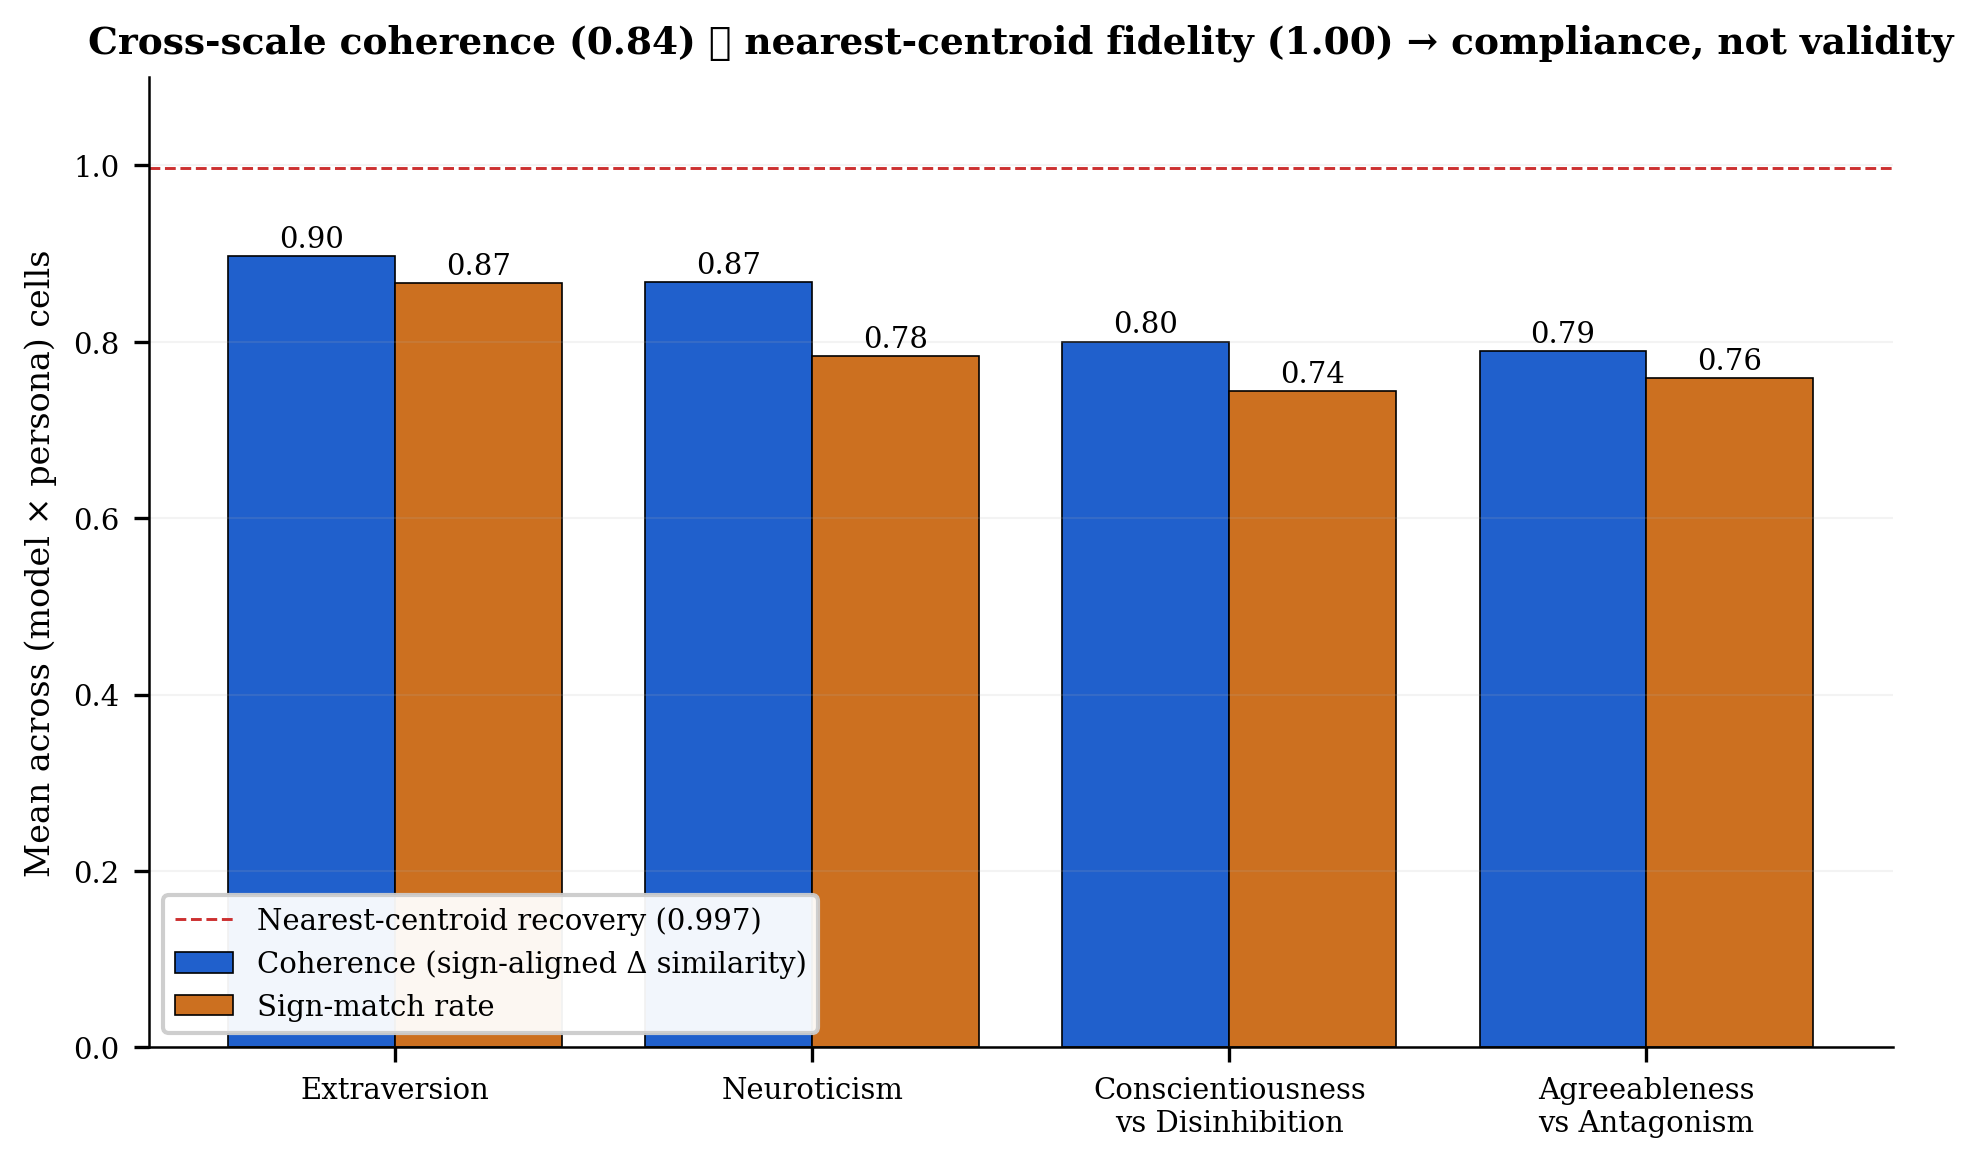
\includegraphics[width=\linewidth]{fig_cross_scale_coherence_by_construct.png}
  \caption{Cross-scale coherence (blue) and sign-match rate (orange) per construct. Far below nearest-centroid fidelity (dashed red).}
  \label{fig:cross_scale_coherence_by_construct}
\end{figure}

Figure~\ref{fig:target_adherence_heatmap} reports per-persona mean target adherence against the LOO empirical centroid and the hand-coded theoretical MBTI target. Empirical adherence averages $0.838$; theoretical adherence averages $0.557$ --- prompted MBTI personas reproduce an empirical pattern that diverges from the textbook descriptions.

\begin{figure}[t]
  \centering
  
\includegraphics[width=0.6\linewidth]{fig_target_adherence_heatmap.png}
  \caption{Per-persona target adherence: LOO-empirical (left column) vs theoretical MBTI mapping (right column).}
  \label{fig:target_adherence_heatmap}
\end{figure}

\subsection{Factorial MBTI main effects}

Figure~\ref{fig:factorial_mbti_main_effects} shows standardised main-effect $\beta$ for the four MBTI axes across the 17 domain scores. Notable cross-axis leakage: EPQR Lie loads heavily on J/P ($\beta = 0.78$); SD3 Narcissism loads heavily on E/I ($\beta = 0.94$).

\begin{figure}[t]
  \centering
  
\includegraphics[width=\linewidth]{fig_factorial_mbti_main_effects.png}
  \caption{Standardised main-effect coefficients of the four MBTI axes on the 17 domain scores.}
  \label{fig:factorial_mbti_main_effects}
\end{figure}

\subsection{EFA robustness and full loadings}

\begin{figure}[t]
  \centering
  
\includegraphics[width=\linewidth]{fig_variance_decomposition_likert_binary.png}
  \caption{Sequential SS decomposition into Model / Domain / Persona / Item / Residual for the Likert (top) and Binary (bottom) composites. The Model slice is barely visible (0.35\% Likert; 0.51\% Binary) — cross-model personality comparisons are statistically negligible.}
  \label{fig:variance_decomposition_likert_binary}
\end{figure}

\begin{table}[t]
\centering
\small
\begin{tabular}{lrrr}
\toprule
Domain & F1 & F2 & F3 \\
\midrule
IPIP Neuroticism                  & $-0.30$       & $\mathbf{+0.72}$ & $+0.39$       \\
IPIP Extraversion                 & $\mathbf{+0.94}$ & $+0.03$       & $+0.29$       \\
IPIP Openness                     & $-0.04$       & $\mathbf{+0.55}$ & $\mathbf{+0.58}$ \\
IPIP Agreeableness                & $+0.05$       & $\mathbf{+0.90}$ & $-0.22$       \\
IPIP Conscientiousness            & $+0.00$       & $-0.04$       & $\mathbf{-0.91}$ \\
SD3 Machiavellianism              & $-0.09$       & $\mathbf{-0.82}$ & $+0.04$       \\
SD3 Narcissism                    & $\mathbf{+0.91}$ & $-0.20$       & $+0.16$       \\
SD3 Psychopathy                   & $+0.38$       & $\mathbf{-0.59}$ & $\mathbf{+0.63}$ \\
ZKPQ Activity                     & $\mathbf{+0.90}$ & $-0.27$       & $-0.12$       \\
ZKPQ Aggression-Hostility         & $+0.48$       & $\mathbf{-0.60}$ & $+0.36$       \\
ZKPQ Impulsive SS                 & $+0.34$       & $+0.08$       & $\mathbf{+0.84}$ \\
ZKPQ Neuroticism-Anxiety          & $-0.27$       & $\mathbf{+0.83}$ & $+0.08$       \\
ZKPQ Sociability                  & $\mathbf{+0.96}$ & $+0.04$       & $+0.13$       \\
EPQR Psychoticism                 & $+0.25$       & $-0.11$       & $\mathbf{+0.88}$ \\
EPQR Extraversion                 & $\mathbf{+0.96}$ & $-0.05$       & $+0.12$       \\
EPQR Neuroticism                  & $-0.04$       & $\mathbf{+0.91}$ & $+0.02$       \\
EPQR Lie                          & $-0.08$       & $+0.07$       & $\mathbf{-0.89}$ \\
\bottomrule
\end{tabular}
\caption{Varimax-rotated factor loadings on the standardised 17-domain matrix ($n=340$). Bold $|loading| > 0.5$. F1 is Extraversion / Sociability; F2 fuses Neuroticism with (inverted) Agreeableness / Machiavellianism; F3 contrasts Conscientiousness with Impulsive Sensation Seeking, Psychoticism, and the Lie scale.}
\label{tab:efa-loadings}
\end{table}

Figure~\ref{fig:efa_loo_robustness} overlays the first-eigenvalue distribution from 20 leave-one-model-out reruns on the full-sample eigenvalue spectrum. All 20 LOO reruns return exactly 3 Kaiser factors.

\begin{figure}[t]
  \centering
  
\includegraphics[width=\linewidth]{fig_efa_loo_robustness.png}
  \caption{Leave-one-model-out replication of the 17-domain EFA. All 20 reruns return exactly 3 Kaiser factors (red dots at $F_1$).}
  \label{fig:efa_loo_robustness}
\end{figure}

\subsection{Default condition baseline}

Figure~\ref{fig:default_persona_classification} shows the nearest-centroid (z-Euclidean) and MBTI-axis classifications of the 20 LLMs under Default. Most models project as ISTJ.

\begin{figure}[t]
  \centering
  
\includegraphics[width=\linewidth]{fig_default_persona_classification.png}
  \caption{Default-condition profile classification: nearest-centroid (blue) and empirical MBTI-axis projection (red). 12/20 LLMs project as ISTJ-like.}
  \label{fig:default_persona_classification}
\end{figure}

\subsection{PIR breakdown}

Figure~\ref{fig:pir_default_vs_mbti} compares Default vs MBTI-mean PIR (left) and reports per-model PIR (right).

\begin{figure}[t]
  \centering
  
\includegraphics[width=\linewidth]{fig_pir_default_vs_mbti.png}
  \caption{Left: Default vs MBTI-mean Pairwise Inconsistency Rate (paired $t = 10.70$, $p < 0.0001$). Right: per-model PIR with overall PIR $= 0.468$.}
  \label{fig:pir_default_vs_mbti}
\end{figure}

\subsection{Per-persona Cronbach's $\alpha$}

Figure~\ref{fig:alpha_per_model_heatmap} shows per-persona $\alpha$ on each IPIP Big Five domain. The reverse-density gradient is preserved under every persona.

\begin{figure}[t]
  \centering
  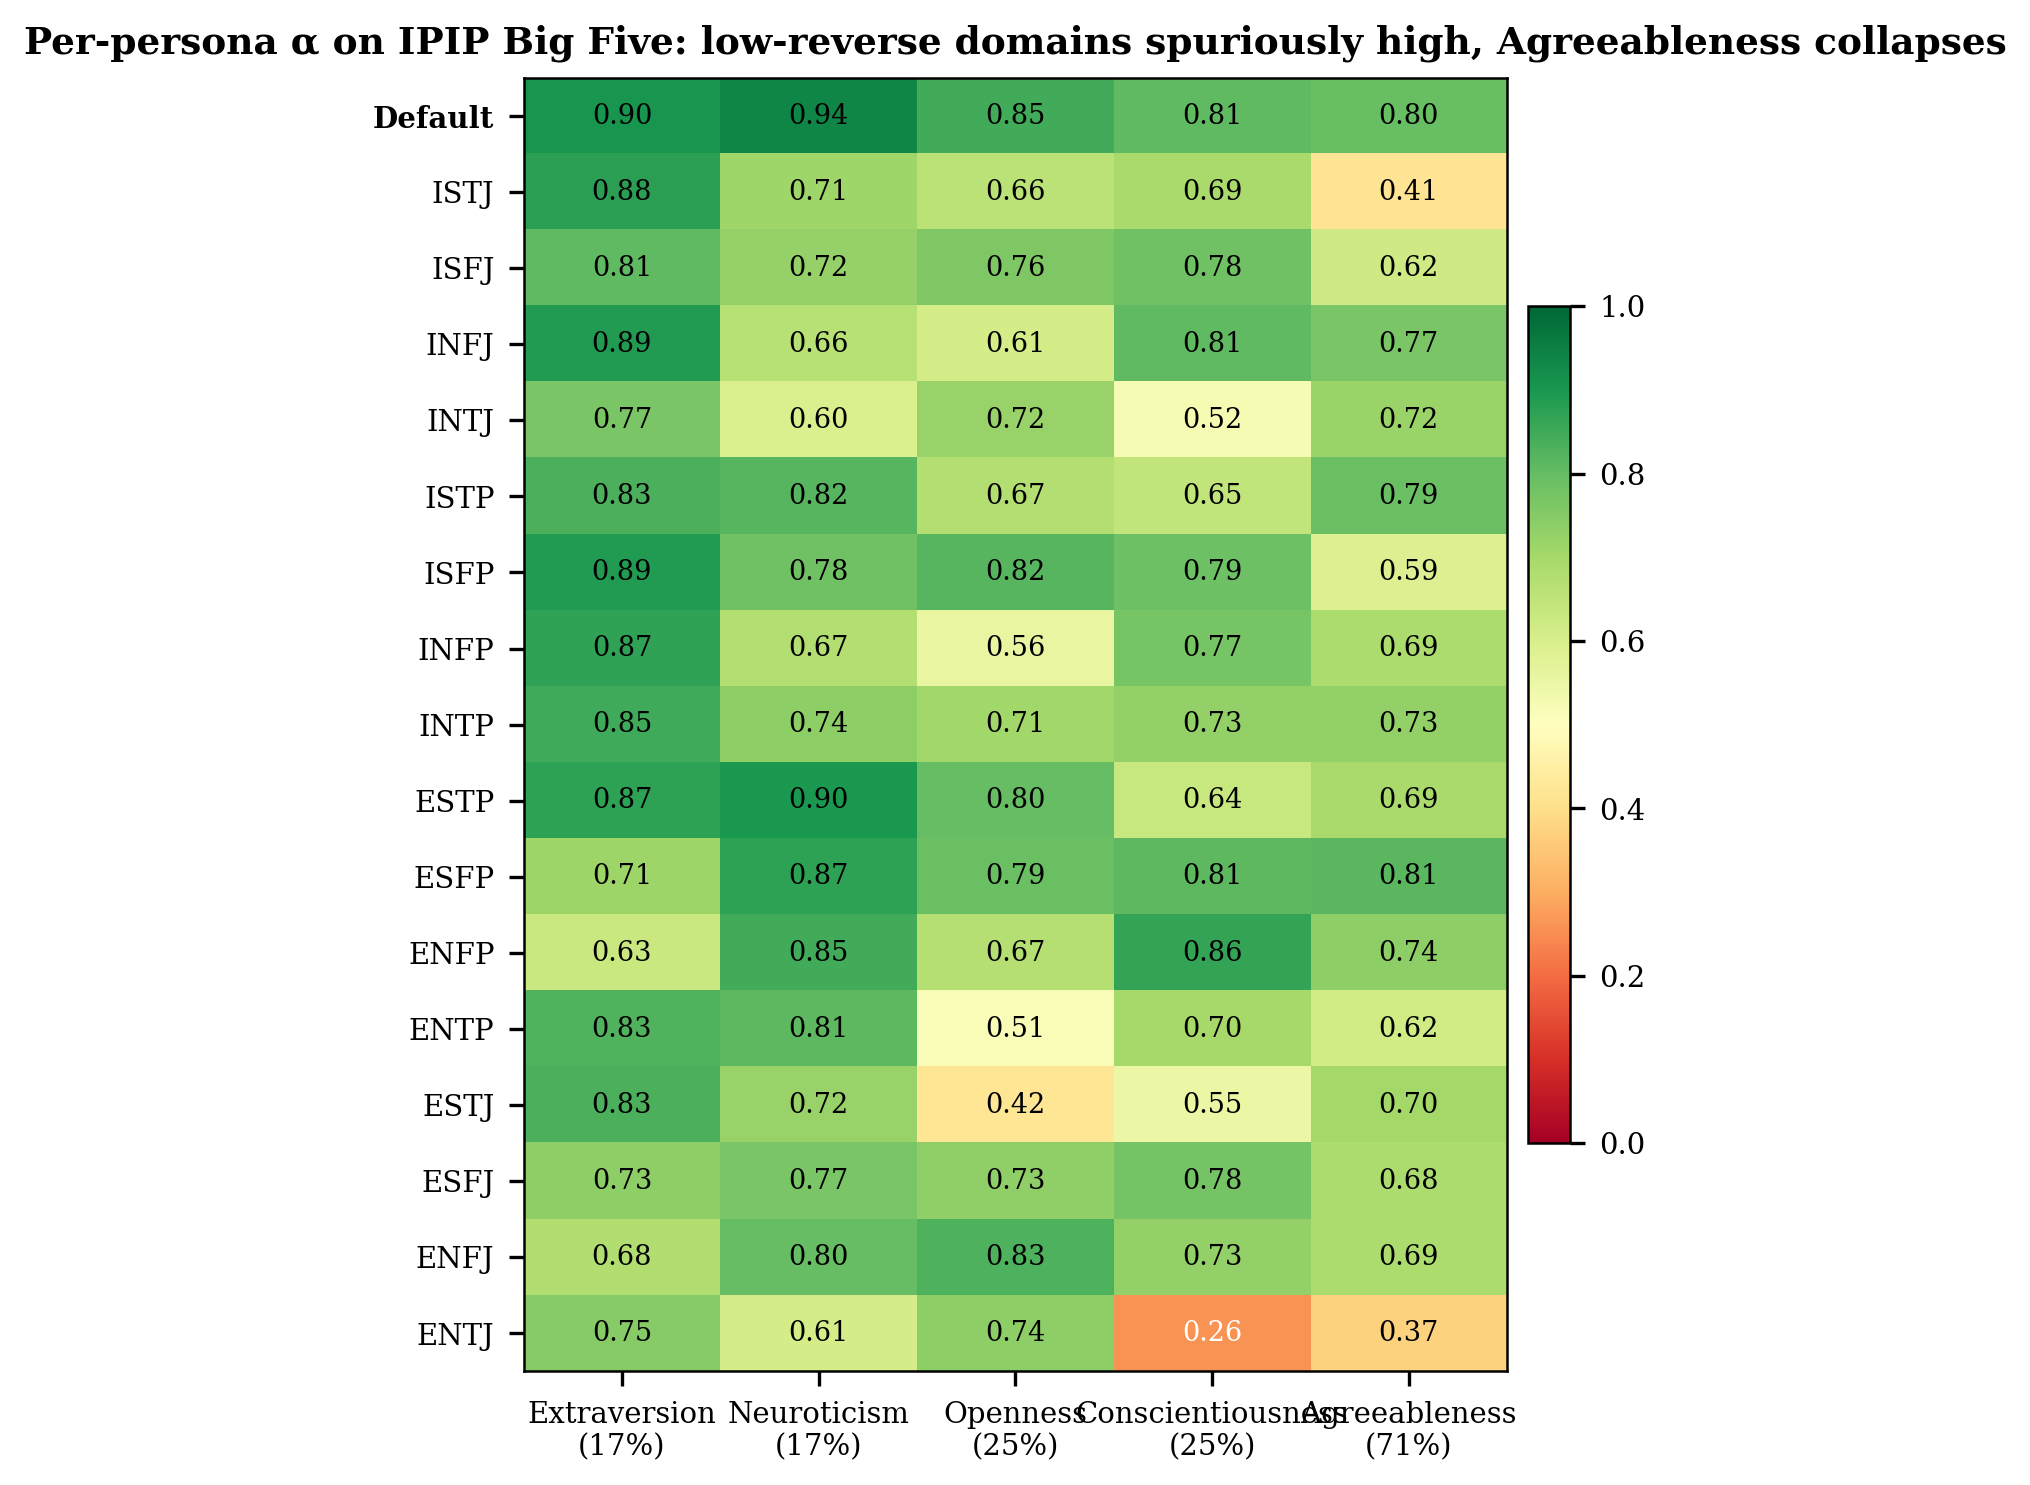
\includegraphics[width=0.7\linewidth]{fig_alpha_per_model_heatmap.png}
  \caption{Per-persona Cronbach's $\alpha$ on IPIP Big Five (columns ordered by reverse-item percentage). Default row in bold. The reverse-density gradient is invariant under role-playing.}
  \label{fig:alpha_per_model_heatmap}
\end{figure}

% ----------------------------------------------------------------------
% Appendix B: DIF
% ----------------------------------------------------------------------

\section{Differential Item Functioning Across Vendor Families}
\label{app:dif}

We tested for DIF across two coarse groupings of vendor families: (i)~Western (Anthropic, OpenAI, Google) vs Chinese (DeepSeek, Alibaba, Zhipu, Moonshot, MiniMax); (ii)~within-vendor-family contrasts using the leave-one-family-out approach. No personality domain shows a statistically significant Western-vs-Chinese gap (Welch's $t$, all $p > 0.16$); the largest effect is $|d| = 0.42$ on Openness. Per-family EFA reruns (one rerun per vendor family) all return exactly 3 Kaiser factors, with first-eigenvalue range $6.71$--$7.18$ across the 8 families.

\begin{table}[t]
\centering
\small
\begin{tabular}{lcrrl}
\toprule
Pair (across 20 models) & Sign & $r_p$ & $p_p$ & OK? \\
\midrule
Neuroticism $\times$ N-Anxiety            & $+$ & $0.64$  & $0.002$ & yes \\
Extraversion $\times$ Sociability         & $+$ & $-0.10$ & $0.670$ & \textbf{NO} \\
Extraversion $\times$ EPQR Extraversion   & $+$ & $0.51$  & $0.020$ & yes \\
Neuroticism $\times$ EPQR Neuroticism     & $+$ & $0.48$  & $0.031$ & yes \\
Agreeableness $\times$ Machiavellianism   & $-$ & $-0.71$ & $0.000$ & yes \\
Agreeableness $\times$ Psychopathy        & $-$ & $-0.81$ & $0.000$ & yes \\
Conscientiousness $\times$ Psychopathy    & $-$ & $-0.73$ & $0.000$ & yes \\
EPQR Psychoticism $\times$ Psychopathy    & $+$ & $0.11$  & $0.646$ & yes \\
\bottomrule
\end{tabular}
\caption{Pearson convergent-validity correlations across the 20 model-level means for 8 pre-specified construct pairs. Sign-match $7/8$, with the single sign reversal on Extraversion $\times$ ZKPQ Sociability.}
\label{tab:convergent}
\end{table}

\begin{table}[t]
\centering
\small
\begin{tabular}{lrrrrr}
\toprule
Strategy            & N & E & O & A & C \\
\midrule
Random              & 0.08 & $-0.01$ & 0.06  & 0.04 & $-0.11$ \\
Pure Acquiescence   & 0.02 & 0.03  & $-0.01$ & 0.10 & $-0.03$ \\
Trait+Acquiescence  & \textbf{1.00} & \textbf{1.00} & \textbf{1.00} & \textbf{1.00} & \textbf{1.00} \\
\midrule
LLM observed        & 0.81 & 0.93 & 0.19  & 0.07 & 0.54 \\
Human (Johnson)     & 0.90 & 0.89 & 0.87  & 0.88 & 0.90 \\
\bottomrule
\end{tabular}
\caption{Cronbach's $\alpha$ per IPIP Big Five domain for three synthetic baselines vs LLM observed and human normative sample.}
\label{tab:synthetic}
\end{table}

\begin{figure}[t]
  \centering
  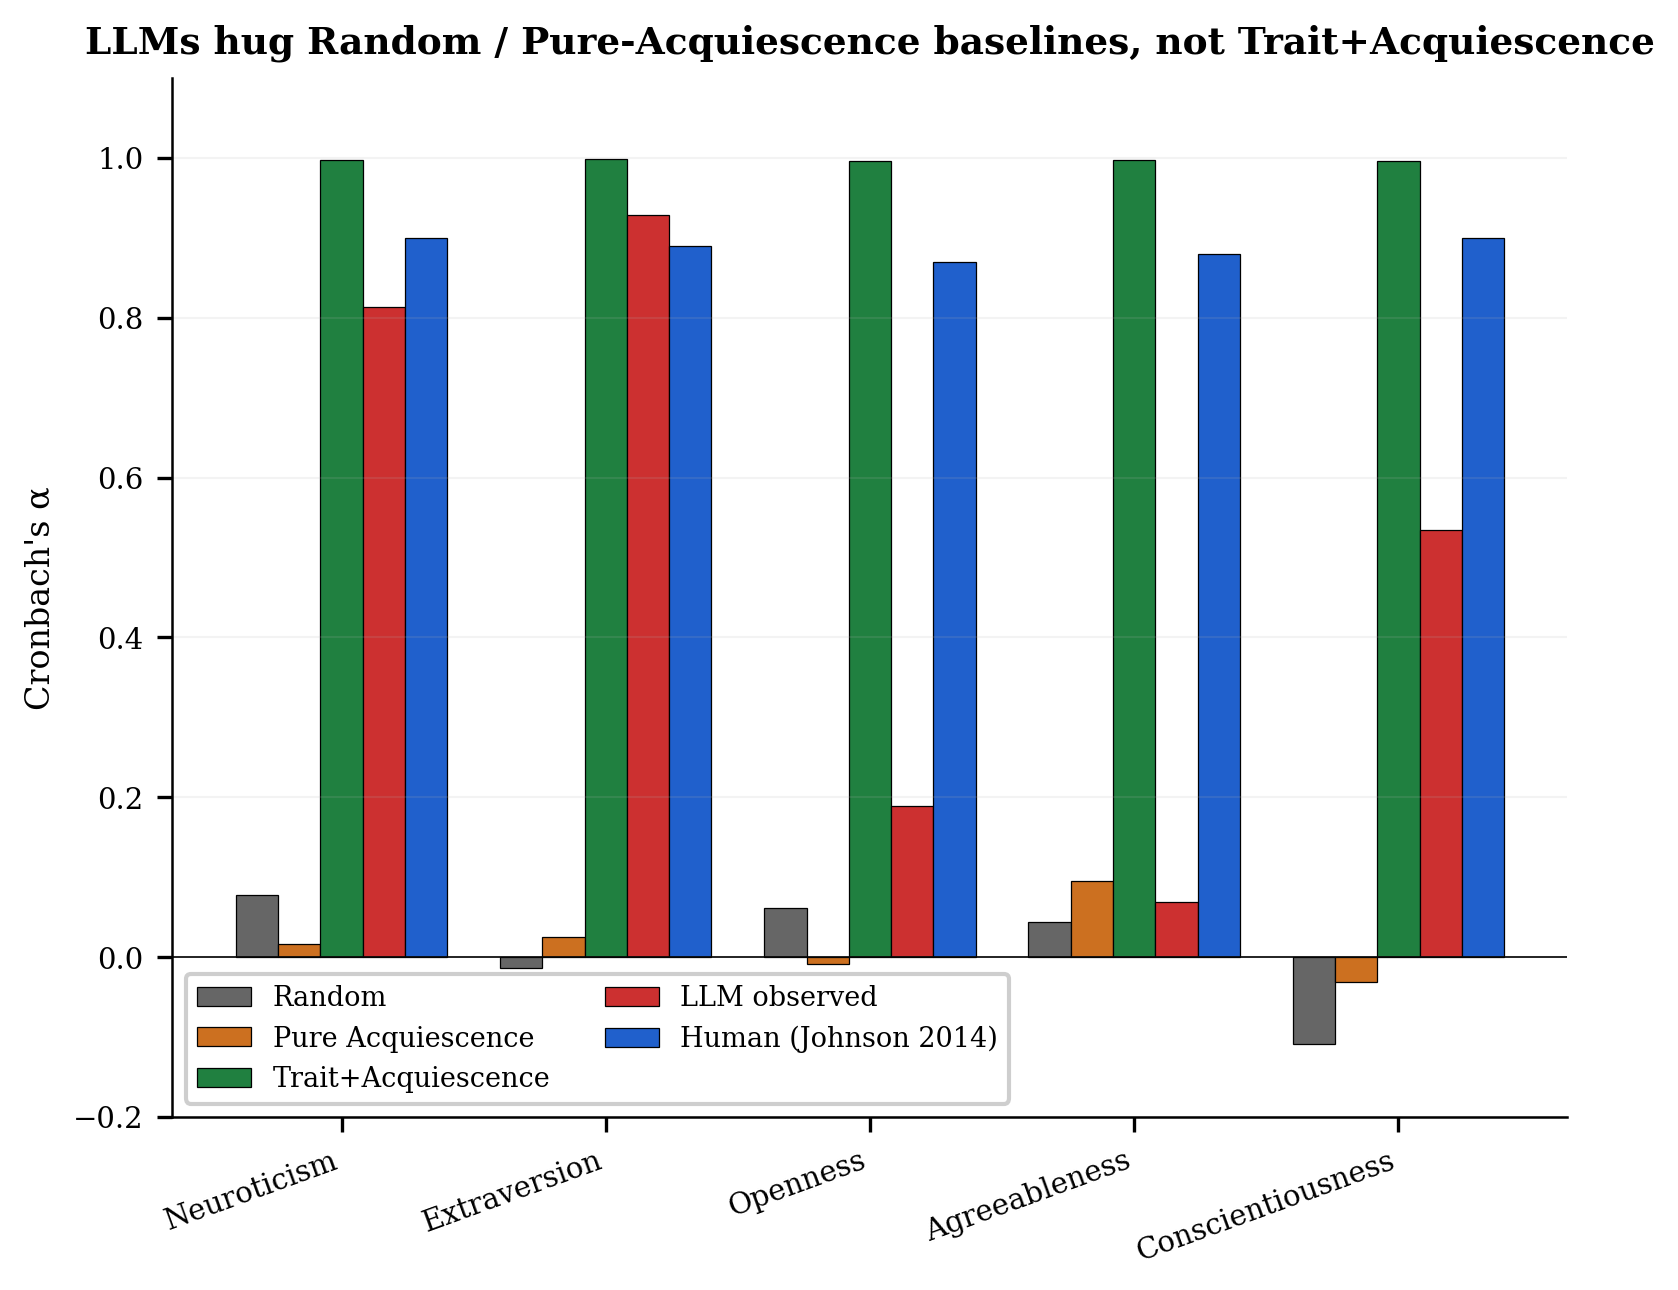
\includegraphics[width=\linewidth]{fig_alpha_synthetic_baseline_calibration.png}
  \caption{Cronbach's $\alpha$ per IPIP Big Five domain for Random, Pure Acquiescence, Trait+Acquiescence, LLM observed, and the human Johnson (2014) baseline.}
  \label{fig:alpha_synthetic_baseline_calibration}
\end{figure}

% ----------------------------------------------------------------------
% Appendix C: Missing-Data
% ----------------------------------------------------------------------

\section{Missing-Data Handling}
\label{app:missing}

\begin{figure*}[t]
  \centering
  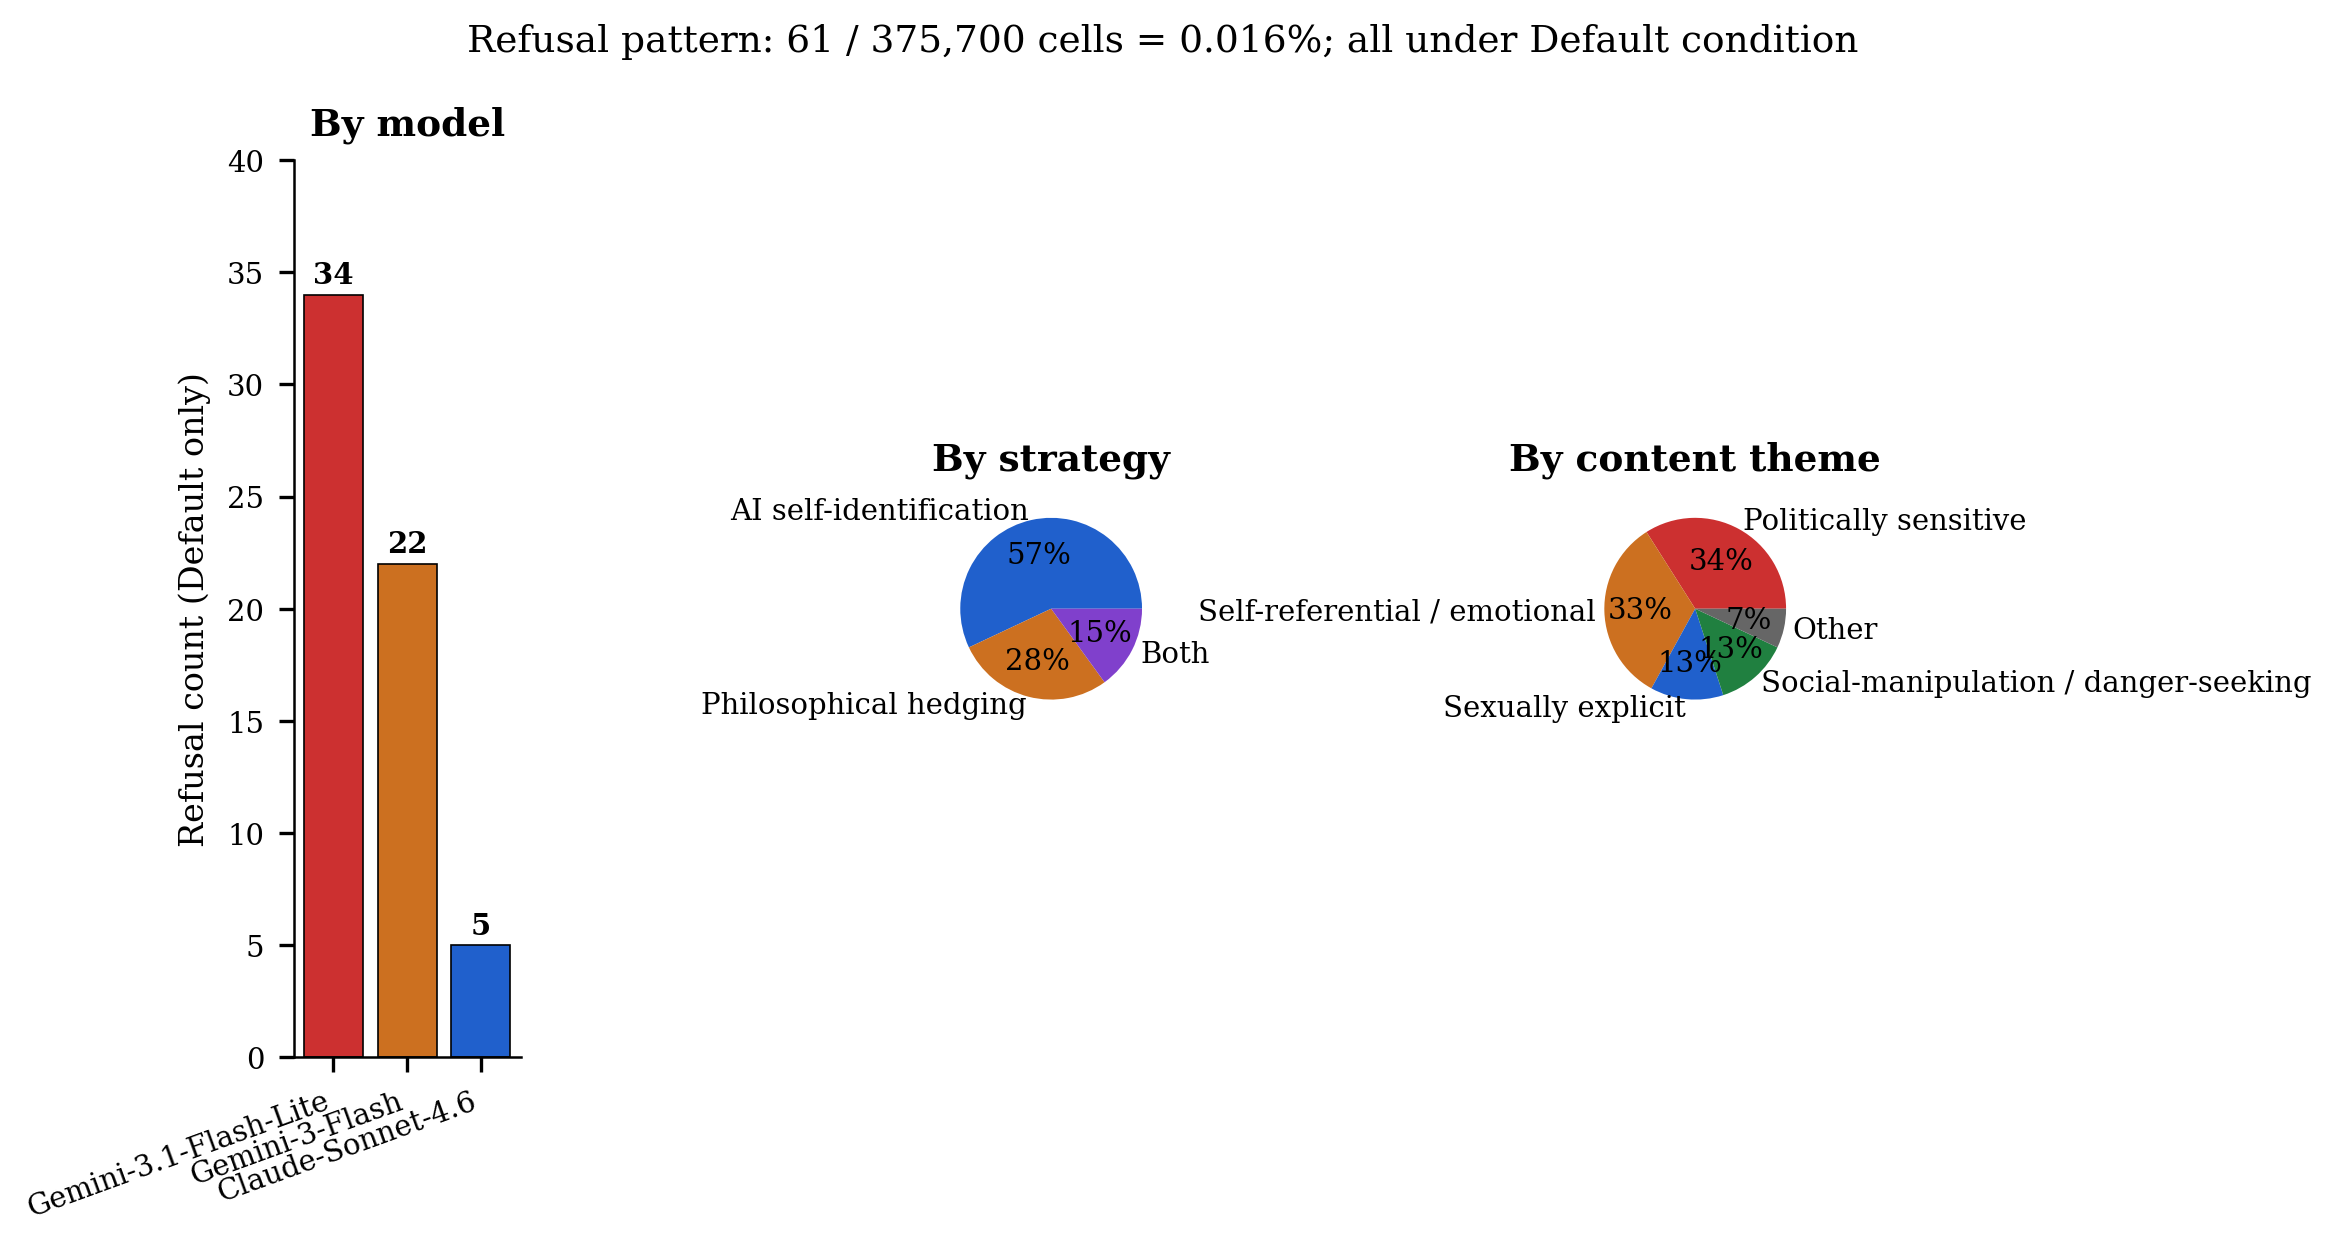
\includegraphics[width=0.95\linewidth]{fig_refusal_breakdown.png}
  \caption{Refusal pattern: 61 / 375{,}700 cells = $0.0162\%$; all under Default. Left: counts by model. Center: refusal strategy. Right: content theme.}
  \label{fig:refusal_breakdown}
\end{figure*}

61 refusals out of 375{,}700 raw API calls ($0.0162\%$) were observed, all under the Default condition (Figure~\ref{fig:refusal_breakdown}). By model: Gemini-3.1-Flash-Lite (34), Gemini-3-Flash-Preview (22), Claude-Sonnet-4.6 (5). By refusal strategy: AI self-identification ($57\%$), philosophical hedging ($28\%$), both ($15\%$). By content theme: politically sensitive ($34\%$), self-referential / emotional ($33\%$), sexually explicit ($13\%$), social-manipulation / danger-seeking ($13\%$). The single most-refused item is SD3-026 (``I enjoy having sex with people I hardly know.'', 8 refusals). Missing cells were filled by per-item mean imputation across remaining models and samples under the same Default condition; the rate is far below any threshold at which the imputation choice could materially affect downstream statistics.

% ----------------------------------------------------------------------
% Appendix D: Within-Sample Consistency
% ----------------------------------------------------------------------

\section{Within-Sample Response Consistency}
\label{app:wsc}

Figure~\ref{fig:within_sample_consistency_by_model} reports per-model within-item SD across the $k=5$ repeated samples on the Likert composite. The total range spans an order of magnitude: Claude-Opus-4.6 ($0.019$, near-deterministic) to DeepSeek-V4-Pro ($0.192$). What looks like a personality difference between Claude and DeepSeek at the profile level is in part a sampling-noise difference. This motivates the multi-seed / multi-temperature recommendation in the Conclusion and is itself a reason to be cautious about cross-model trait comparisons.

\begin{figure}[t]
  \centering
  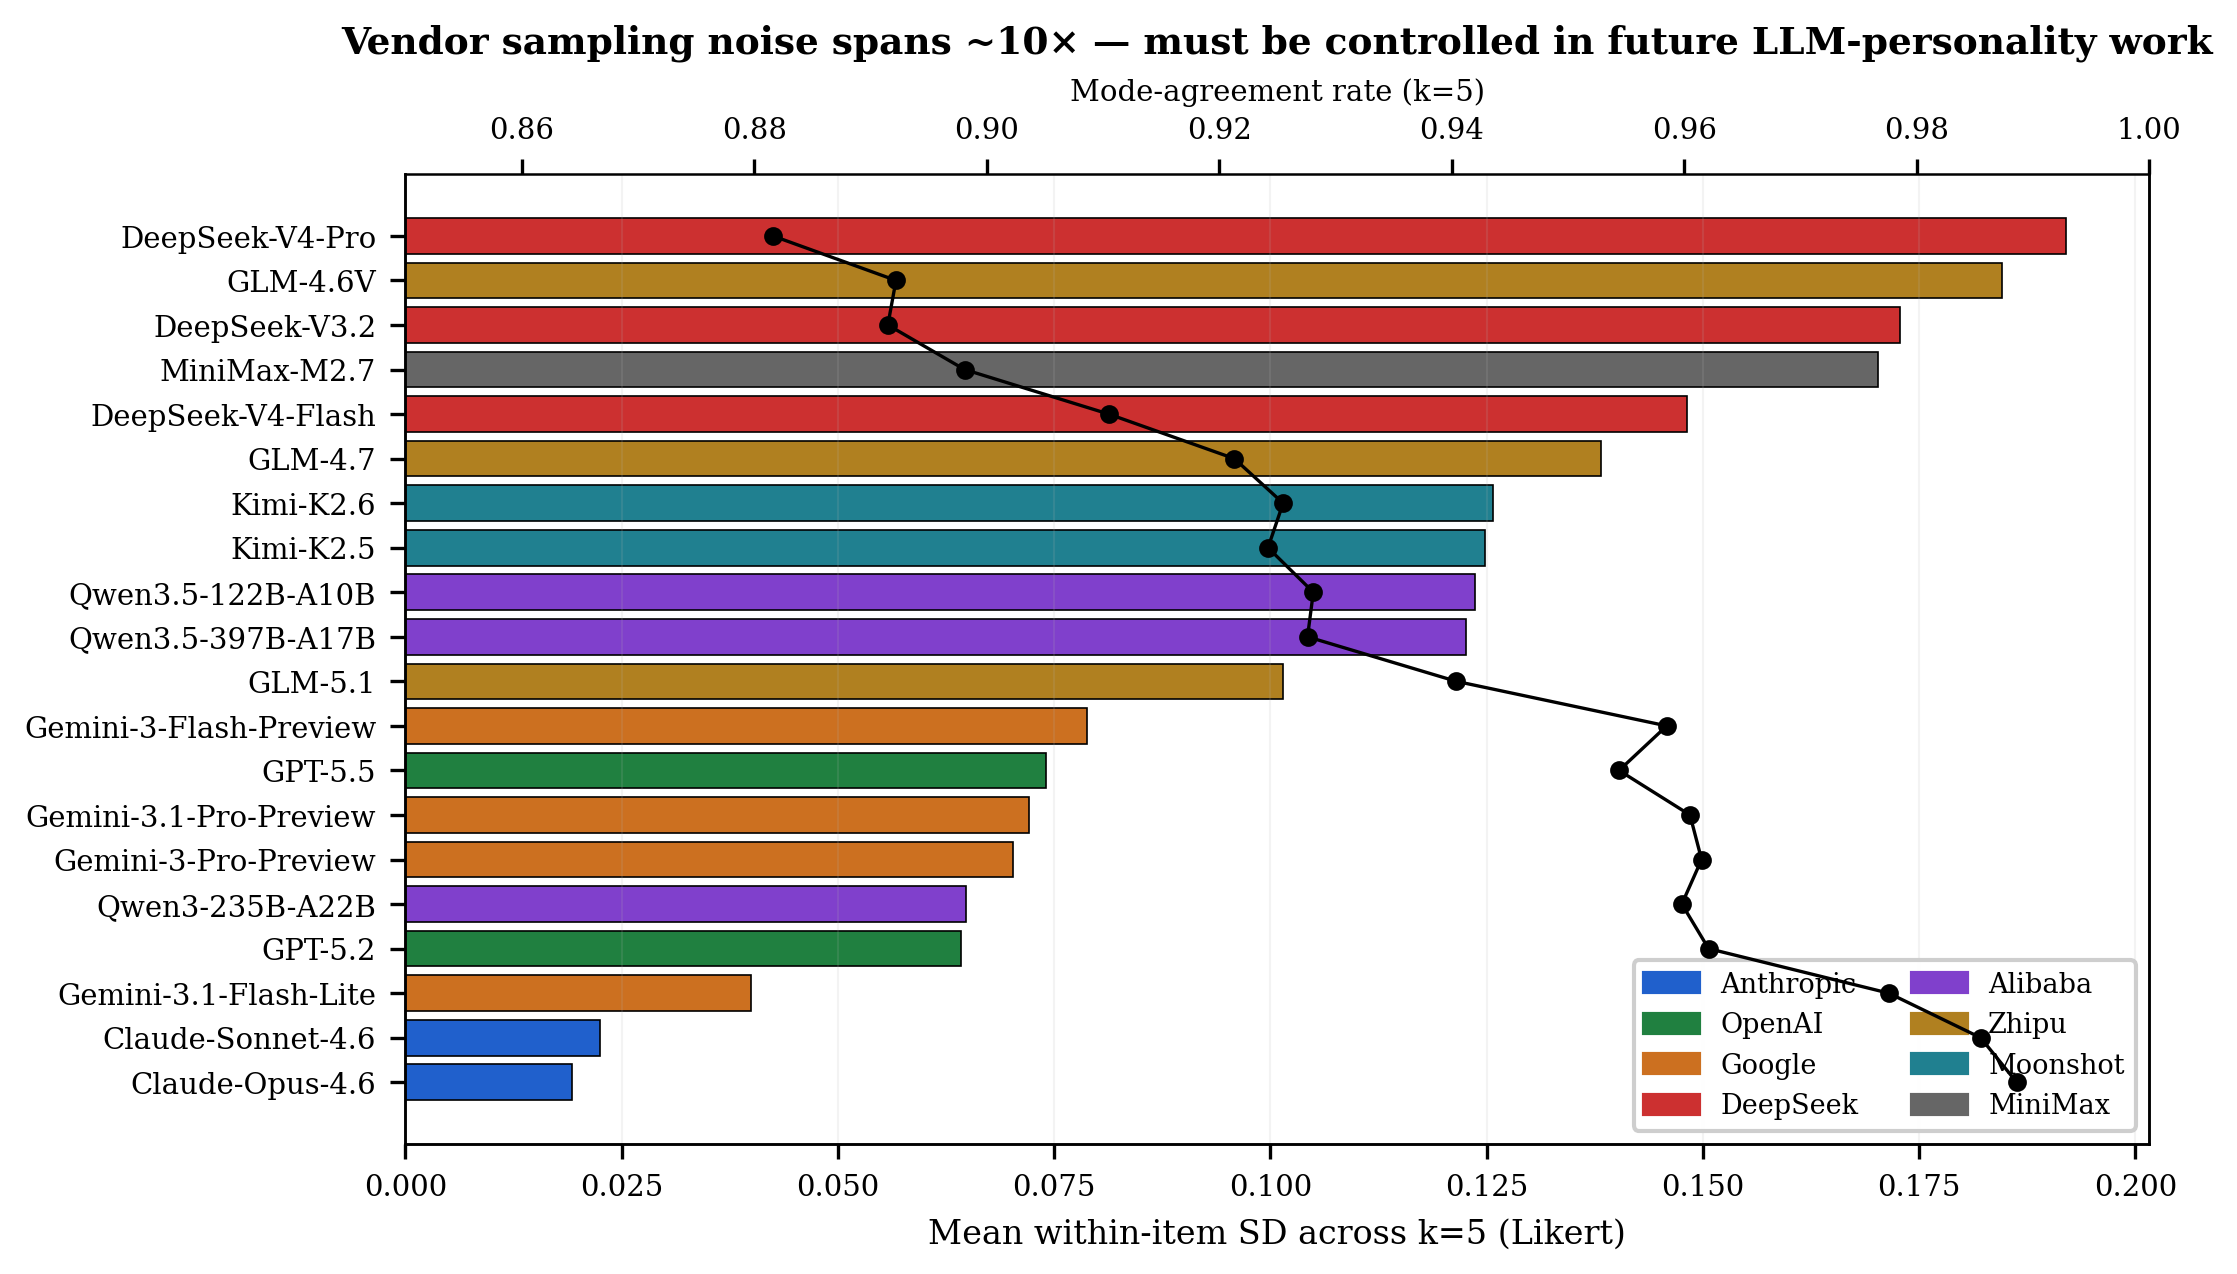
\includegraphics[width=\linewidth]{fig_within_sample_consistency_by_model.png}
  \caption{Within-sample stability across $k=5$ repeats per model (Likert items). Bars: mean within-item SD coloured by vendor family. Line: mode-agreement rate on the secondary axis. Vendor sampling noise spans ${\approx}10\times$.}
  \label{fig:within_sample_consistency_by_model}
\end{figure}

\textbf{Per-persona stability.} Mean within-item SD per persona ranges from $0.081$ (ISFJ) to $0.118$ (ISTP); the Default condition is the noisiest of all at $0.205$. Persona prompts therefore reduce response stochasticity rather than increasing it --- giving the model a coherent character to inhabit reduces the alignment-vs-honesty tension that drives Default-condition jitter.

\textbf{Binary scales.} On binary scales the picture is sharper: mean within-item SD is $0.037$ on ZKPQ true/false and $0.032$ on EPQR yes/no, with mode-agreement rates above $0.99$ on most (model, persona) cells.

% ----------------------------------------------------------------------
% Appendix E: Sample-count convergence
% ----------------------------------------------------------------------

\section{Sample-count convergence}
\label{app:convergence}

To confirm that $k{=}5$ samples per cell suffice, we recompute the three headline diagnostics using only the first $k \in \{1,2,3,4,5\}$ samples and correlate each against the $k{=}5$ baseline across the 20 models (Spearman $\rho$). For Cronbach's $\alpha$, four of the five IPIP domains exceed $\rho{=}0.98$ by $k{=}3$; Openness, the most reverse-heavy domain ($38\%$), reaches $\rho{=}0.94$ at $k{=}3$ and $0.97$ at $k{=}4$. For the Pairwise Inconsistency Rate, $\rho(k{=}3,k{=}5)=0.98$ (mean absolute error $0.014$; $0.008$ at $k{=}4$). The EFA factor structure is perfectly stable: $k{=}1,3,5$ each yield exactly three factors under both the Kaiser criterion and parallel analysis, with near-identical eigenvalues (top three $6.84/4.33/3.00$, $6.96/4.32/3.06$, $6.97/4.33/3.07$). $k{=}3$ is therefore sufficient and $k{=}5$ conservative; no main conclusion depends on the sample count.

\end{document}
